\documentclass{report}

\usepackage{amsmath}
\usepackage[inlinechap]{settings/fncystyle}

\input{preamble}
\input{macros}
\input{letterfonts}

\usepackage[indent=0pt]{parskip}

\renewcommand{\chaptername}{Capitolo}
\renewcommand{\contentsname}{Indice}

\title{\Huge\textbf{{Appunti Cosmologia 2}}}
\author{Giacomo Galliani, corso del prof. L. Guzzo}
\date{Anno accademico 2025-2026}

\begin{document}

\maketitle
\newpage% or \cleardoublepage
% \pdfbookmark[<level>]{<title>}{<dest>}
\pdfbookmark[section]{\contentsname}{toc}
\tableofcontents
\pagebreak

\chapter{Aspetti fondamentali e struttura a grande scala}

\section{Metrica di Robertson-Walker}

In relatività generale, una volta che si assume il \emph{principio cosmologico}, ovvero si assume che l'universo sia lo stesso in tutte le direzioni e che non siamo in un punto eccezionale, la metrica diventa massimamente simmetrica, ed in particolare diventa la metrica di FRW. Questa è data da 

\begin{equation}
    ds^2 = -c^2dt^2 + a^2(t)d\Omega_k^2
\end{equation}

Dove $d\Omega_k^2$ indica la metrica sullo spazio sferico, piatto, o iperbolico (e.g per lo spazio piatto $d\Omega_0^2= dx^2 + dy^2 + dz^2 = dr^2 + r^2(d\theta^2 + \sin^2\theta d\varphi^2)$). \\
In questo contesto altamente simmetrico le eq. di Einstein si riducono a due equazioni per il fattore di scala $a = a(t)$, dette le eq. di Friedman. \\
Sebbene la loro dimostrazione si svolga in relatività generale, è possibile ottenerle con ragionamenti classici (ed euristici): \\
Consideriamo un fluido omogeneo sferico, con densita $\rho$, autogravitante, in espansione: \\


\begin{multicols}{2}

Considero un punto di massa $m$, sulla superfice della sfera. Per effetto dell'espansione di questa, al momento di interesse il punto ha una velocità $\vec{v}$. Chiaramente la massa contenuta dentro il raggio $R$ è data da 

\begin{equation}
    M(<R) = \frac{4}{3}\pi \rho R^3
\end{equation}

\columnbreak

% Imposto vista 3D
\tdplotsetmaincoords{0}{0}

\begin{tikzpicture}[tdplot_main_coords]

  % Raggio della sfera
  \def\r{2}

  % Disegno la sfera
  \shade[ball color=gray!40, opacity=0.9] (0,0,0) circle (2cm);

  % Definisco le coordinate del punto sulla superficie (theta = longitudine, phi = latitudine)
  \tdplotsetcoord{P}{\r}{270}{180} % (Nome, raggio, angolo phi, angolo theta)
  \tdplotsetcoord{Q}{1.1\r}{270}{180}


    \draw[->, thick, black] (Q) -- (P) node[midway, above] {$\vec{v}$};
  % Segno il punto

    \fill[black] (Q) circle (2pt) node[below] {$m$};

    %ora invece mi occupo di disegnare il raggio 
    \tdplotsetcoord{O}{0}{0}{0}
    %\fill[black] (O) circle (1pt) node[below] {$Origin$};
    \tdplotsetcoord{R}{\r}{90}{270}
    \draw[->, thick, dashed, black] (O) -- (R) node[midway, right]{$R$}; 

\end{tikzpicture}

\end{multicols}

\vspace{0.5cm}
Possiamo allora scrivere l'energia potenziale e cinetica del punto: 

\[\begin{cases}
    V = - \frac{4}{3}m\pi R^2 \rho G \\
    K = \frac{1}{2}m\dot{R}^2
\end{cases}\]

Imponendo la condizione $K + V = cost.$, otteniamo \\

\begin{equation}
    \dot{R}^2 - \frac{8\pi G \rho}{3}R^2 = cost. 
\end{equation}

Eseguendo il conto corretto in GR, si scopre che $cost. = -c^2$. Scrivendo inoltre $R(t) = a(t)R_0$, e notando che $k = R_o^{-2}$ è la curvaura della sfera, arriviamo a scrivere la 1° eq. di Friedman, 

\begin{tcolorbox}[colback=gray!15, colframe=black, boxrule=1pt]
\begin{equation}
    \label{first_friedman}
    \left(\frac{\dot{a}}{a} \right)^2 = \frac{8\pi \rho G}{3} - \frac{kc^2}{a^2} 
\end{equation}
\end{tcolorbox}

Il rapporto $\dot{a}/a = H(a)$ è detto \emph{parametro di Hubble}, e la \emph{costante di Hubble} è il parametro di Hubble calcolato oggi, $H_0 = H(a)|_{a = a_0 = 1} = 70 km/s/Mpc$. \\
Notiamo inoltre che l'eq. \ref{first_friedman} ai giorni nostri si può scrivere 

\begin{equation}
    H_0^2 = \frac{8\pi G\rho_0}{3} - kc^2
\end{equation}

Che definisce una densità critica affinchè la metrica sia piatta (ovvero valga $k=0$), data da

\begin{equation}
    \label{critical_density}
    \rho_{0, c} = \frac{3H_o^2}{8\pi G}
\end{equation}


Sempre da ragionamenti classici, si può ottenere una importante legge di conservazione. Se pensiamo al nostro universo come un oggetto termodinamico \emph{isolato}, la prima legge della termodinamica ci dice che 

\begin{equation}
    \label{first_principle}
    dU = \delta L = -pdV
\end{equation}

è comodo definire una densità di energia $\epsilon$, t.c. $U = \epsilon V$. Per un universo sferico di raggio $R$, chiaramente 

\begin{equation}
    \label{universe_volume}
    V = \frac{4}{3}\pi a^3 R_0^3
\end{equation}

Dividendo per $da$ l'eq. \ref{first_principle}, otteniamo

\begin{equation}
    \frac{dU}{da} = \frac{\partial U}{\partial \epsilon}\frac{d\epsilon}{da} + \frac{\partial U}{\partial V}\frac{dV}{da} = V\frac{d\epsilon}{da} + \epsilon\frac{dV}{da} = -p\frac{dV}{da} 
\end{equation}

Derivando la \ref{universe_volume} otteniamo che

\begin{equation}
    \frac{dV}{da} = 4\pi R_0^3 a^2
\end{equation}

Otteniamo così

\begin{equation}
    \frac{a}{3}\frac{d\epsilon}{da} = -(\epsilon + p)
\end{equation}

Passando dalla densità di energia alla denistà di materia, troviamo finalmente 

\begin{tcolorbox}[colback=gray!15, colframe=black, boxrule=1pt]
\begin{equation}
    \label{coservation_friedman}
    \frac{d\rho}{da} = -\frac{3}{a}\left[\rho +  pc^2\right]
\end{equation}
\end{tcolorbox}

L'eq. \ref{coservation_friedman} è importante perchè nota la relazione $p = p(\rho)$ (detta \emph{equazione di stato}), è possibile determinare $\rho(a)$. Vediamo alcuni esempi rilevanti in cosmologia e come questi ci permettano di identificare delle ere in cui particolari tipi di energia sono dominanti. \\

Spesso l'eq. di stato ha la forma $p_i = w_i\rho_ic^2$: in questo caso, la sol. della \ref{coservation_friedman} è data semplicemente da 

\begin{equation}
    \rho_i(a) = \rho_{0, i}a^{-3(1 + w_i)}
\end{equation}

\vspace{0.5cm}
Per la \emph{materia}, vale $w_m = 0$, che implica $\rho_m(a) = \rho_{m,0}a^{-3}$.  \\

Per la \emph{radiazione} (o la materia relativistica), $w_\gamma = 1/3 \rightarrow \rho_\gamma (a) = \rho_{\gamma , 0}a^{-4}$. \\

Infine, per \emph{l'energia oscura}, $w_\Lambda = -1 \rightarrow \rho_\Lambda(a) = \rho_{\Lambda, 0} $. \\

Facciamo dunque un diagramma per le varie densità delle specie, all'espandersi dell'universo (per comodità in scala logaritmica): \\

\begin{multicols}{2}

\begin{tikzpicture}[scale=0.7]
    \begin{axis}[
        xmin = 0, xmax = 2,
        ymin = 0, ymax = 2,
        xlabel = {$a(t)$},
        ylabel = {$\rho_i(a)$},
        grid = both,                % griglia
        grid style = {dashed, gray!30},
        axis lines = left,          % assi più puliti
        legend style={at={(0.98,0.98)},anchor=north east}, % legenda in alto a dx
        legend cell align={left},
        thick, % linee più spesse
    ]
        \addplot[color=red,   domain=0:2]{1} node[pos=0.85, above, sloped] {\small $\rho_\Lambda$};
        \addplot[color=blue,  domain=0:2]{2-x} node[pos=0.7, below, sloped] {\small $\rho_\gamma$};
        \addplot[color=orange,domain=0:2]{1.75 - x/2} node[pos=0.6, above, sloped] {\small $\rho_m$};
        
        % In alternativa alle etichette "sulle curve" puoi usare la legenda:
        % \addlegendentry{$\rho_\Lambda$}
        % \addlegendentry{$\rho_m$}
        % \addlegendentry{$\rho_r$}

        \begin{pgfonlayer}{background}
            \fill[blue!10]  (axis cs:0,0)   rectangle (axis cs:0.5,2);
            \fill[green!10] (axis cs:0.5,0) rectangle (axis cs:2,2);
        \end{pgfonlayer}


        
        % --- Note sul grafico ---
        \node at (axis cs:0.25, 0.5) {\small Era della};
        \node at (axis cs:0.25, 0.4) {\small radiazione};
        \node at (axis cs:1.25,1.8) {\small Era della materia};
    \end{axis}
\end{tikzpicture}

\columnbreak

Dunque, nell'universo giovane la radiazione era il contributo più rilevante. Questo periodo è detto \emph{era della radiazione}. Esiste inoltre un'epoca dove $\rho_\gamma = \rho_m$, detto periodo dell'equivalenza, prima ancora della riconbinazione. Dopo quest'epoca, si parla di \emph{era della materia}. Importante è notare che adesso siamo un'epoca dove $\rho_\Lambda > \rho_m$, seppure siano nello stesso ordine di grandezza. 

\end{multicols}

La seconda eq. di Friedman è invece data da

\begin{tcolorbox}[colback=gray!15, colframe=black, boxrule=1pt]
\begin{equation}
    \label{second_friedman}
    \frac{\ddot{a}}{a} = -\frac{4\pi G}{3}\left(\rho + \frac{3p}{c^2} \right)
\end{equation}
\end{tcolorbox}

Come vedremo, l'eq. \ref{second_friedman} è importante per comprendere l'espansione accellerata dell'universo. \\
Le eq. di Friedman (\ref{first_friedman}, \ref{second_friedman}) possono essere scritte in un modo equivalente, introducendo i parametri adimensionali $\Omega_i = \rho_i/\rho_c$, con $\rho_c$ la densità critica, data da \ref{critical_density}. 

Infatti, la \ref{first_friedman} si può scrivere in termini del parametro di Hubble: 
\begin{equation}
    H^2 = \frac{8\pi G}{3}\left[\rho_{m, 0}a^{-3} +  \rho_{\gamma, 0}a^{-4} + \rho_\Lambda  \underbrace{- \frac{3}{8\pi G}k\frac{c^2}{a^2}}_{:= \rho_ka^{-2}}\right]
\end{equation}

Moltiplicando e dividendo il lato destro per $H_0^2$, riconoscendo l'inverso della densità critica possiamo scrivere 

\begin{equation}
    H(a)^2 = H_0^2\left[\Omega_{m,0}a^{-3} + \Omega_{\gamma,0}a^{-4} + \Omega_{\Lambda} + \Omega_{k,0}a^{-2}\right]
\end{equation}

Allo stesso modo facciamo per l'eq. \ref{second_friedman}, che possiamo scrivere ai giorni nostri (trascurando i contributi infinitesimi di $\Omega_\gamma \, , \Omega_k$), come 

\begin{equation}
    \frac{\ddot{a}}{a} = - \frac{H_0^2}{2}\left[\Omega_{m, 0}a^{-3}  - 2\Omega_{\Lambda}\right]
\end{equation}

I dati sperimentali ci dicono che $\Omega_{m,0} \approx 0,3 \, , \Omega_{\Lambda,0} \approx 0,7$, il che mostra $(\ddot{a}/a) > 0$. \\

Vediamo ora una formula alternativa della metrica FRW, che dipende esplicitamente dalla metrica. Consideriamo la seguente parametrizzazione della sfera: 

\begin{multicols}{2}
    \tdplotsetmaincoords{0}{0}
    \begin{tikzpicture}[tdplot_main_coords]

    % Raggio della sfera
    \def\r{2}

% Disegno la sfera
    \shade[ball color=gray!10, opacity=0.9] (0,0,0) circle (2cm);

    %ora invece mi occupo di disegnare il raggio 
    \tdplotsetcoord{O}{0}{0}{0}
    %\fill[black] (O) circle (1pt) node[below] {$Origin$};
    \tdplotsetcoord{R}{\r}{90}{270}
    \draw[->, thick, dashed, black] (O) -- (R) node[midway, right]{$R$}; 

    \tdplotsetcoord{P}{\r}{315}{-45}
    \fill[black] (P) circle (2pt) node[below] {$P$};
    \tdplotsetcoord{N}{\r}{90}{90}
    \fill[black] (N) circle (2pt) node[below] {$N$};
    \tdplotsetcoord{O}{0}{0}{0}

    \draw[-, thick, black] (P) -- (N) node[midway, right]{$\rho$};
    \draw[-, dashed, thick, black] (O) -- (P); 
    \draw[-, thick, dashed, black] (O) -- (N) node[pos=0.25, left]{$\beta$}; 

    \tdplotsetcoord{A}{\r}{280}{0}
    %\fill[black] (A) circle (2pt) node[below] {$A$};
    \tdplotsetcoord{B}{\r}{320}{20}
    %\fill[black] (B) circle (2pt) node[below] {$B$};
    \draw[-, dashed, thick, black] (O) -- (A); 
    \draw[-, thick, dashed, black] (O) -- (B) node[pos=0.25, left]{$\alpha$};
    
\end{tikzpicture}

\columnbreak

Fissiamo un punto, ad esempio il polo nord $N$, e prendiamo come coordinata la lunghezza dell'arco che collega un punto generico $P$ e il polo. Definiamo anche i due angoli $\alpha, \beta$, come in figura. La metrica in queste coordinate si legge 

\begin{equation}
    d\ell^2 = d\rho^2 + \rho^2\sin^2(\beta)d\alpha^2
\end{equation}

Riconoscendo però che $\beta = \rho/R$, si ottiene quindi 

\end{multicols}

\begin{equation}
    d\ell^2 = d\rho^2 + \rho^2\sin^2{(\rho/R)}d\alpha^2
\end{equation}

Viene dunque naturale definire la nuova coordinata $x = R\sin(\rho/R)$ (che corrisponde semplicemente alla proiezione sul piano $(x,y)$ dell'arco), in termini dei quali la metrica si scrive 

\begin{equation}
    \label{FRW_Longair}
    d\rho^2 = \frac{dx^2}{1-kx^2} \rightarrow ds^2 = c^2dt^2 - \frac{dx^2}{1-kx^2} -x^2d\Omega^2 
\end{equation}

Dove, come promesso, $k= R^{-1}$ è la curvatura del sistema. Sebbene sia stata ricavata come la metrica relativizzata sulla sup. di una sfera, la eq. \ref{FRW_Longair} può essere utilizzata anche per spazi a curvatura nulla (euclidei) oppure a curvatura negativa (iperbolici). \\

Talvolta (e.g. nel libro di Weinberg), la metrica \ref{FRW_Longair} è invece scritta in modo tale che $k= \pm1, 0$. Questo si ottiene perchè semplicemente il modulo della curvatura viene incluso nel fattore di scala. Chiaramente, in ogni situazione è importante capire di che metrica si sta parlando così da non sbagliare i conti. 

\section{Distanze in Cosmologia}

In cosmologia è possibile fare diverse misure di distanza. Una scelta possibile, e naturale, è la distanza comovente: questa è proprio la distanza $r$ che compare nella metrica di Robertson-Walker. Allora il fotone seguirà una geodetica $ds^2 = 0$, e assumendo senza ledere la generalità che il fotone si muova in direzione radiale, varrà $0 = cdt - dr$, che integrato ci dice 

\begin{equation}
    r = c\int_{t_o}^t\frac{dt^{'}}{a(t^{'})}
\end{equation}


Un'altro possibile metodo è la distanza angolare. Se sono nello spazio euclideo, la distanza di un oggetto di nota lunghezza $\ell$ dato un angolo di osservazione $\theta$ è dato da
\begin{equation}
    D_A = \frac{\ell}{\theta}
\end{equation}

Quando la metrica è quella di Roberston-Walker, come cambia questa definizione? Avremo

\begin{equation}
    D_A = R\sin{\frac{r}{R}}a = \frac{D}{1+z}
\end{equation}


\section{Red-shift Surveys e la funzione di autocovarianza}

A partire dagli anni '50, si cominciarono ad avere delle misure sistematica del numero di oggetti (per unità di superficie) extragalattici. Negli anni '70 si cominciarono ad eseguire calcoli e in particolare calcolare le \emph{funzioni di correlazione} relativi a queste osservazioni. A partire dagli anni '90, le misure divennero automatizzate ed adesso lo strumento più importante in questo settore è DESI (Dark Energy Spectroscopic Instrument). Quello che si osservava nelle prime misure erano dei grandi ammassi di galassie, soprattutto \emph{l'ammasso della vergine} e \emph{la chioma di Berenice}. Questo sembrava contraddire l'ipotesi fondamentale di omogeneità. Il problema era che questi strumenti non riuscivano a guardare più lontano: le misure odierne confermano l'omogeneità dell'universo, su scale \emph{molto grandi}. \\

Vediamo ora come possiamo fare della statistica oppure delle previsioni teoriche lavorando su delle  red-shift surveys. Immagino di avere a che fare con $\bar{n}(\vec{x})$, ovvero la densità numerica di una survey, oppure $T(\theta, \varphi)$ del CMB. Una teoria non può predirre queste funzioni, ma può invece predirre delle quantità stocastiche, trattando $\bar{n}(\vec{x}), \, T(\theta, \varphi)$ come dei \emph{campi stocastici}. \\

Se $\rho = \rho (\vec{x})$ è una variabile stocastica, allora questa avrà una certa distribuzione di probabilità $P= P(\rho)$, e il valore di aspettazione di $\rho$ sarà dunque dato da

\begin{equation}
    <\rho> = \int d\rho \rho P(\rho )
\end{equation}

Così come il suo n-esimo momento sarà dato da 

\begin{equation}
    <\rho^n> = \int d\rho \rho^n P(\rho )
\end{equation}

E la sua varianza 
\begin{equation}
    \sigma^2 = <\rho^2> - (<\rho>)^2
\end{equation}

Qui vi è un punto particolarmente delicato: l'integrale in $d\rho$ in tutti questi casi non è fatto su tutto lo spazio, ma è fatto sullo stesso punto dello spazio, in tutte le possibili realizzazioni del nostro universo. Dalla definizione dunqe non è ovvio capire come sia possibile per noi calcolare questi valori di aspettazione, visto che disponiamo di un solo universo. La via d'uscita da questo enorme problema è \emph{l'ipotesi ergodica}. Grazie a questa, posso passare dalle medie sugli universi a medie spaziali. Questa è valida solo se i campioni che prendo sono "fair samples of the universe" (nelle parole di Peebles), ovvero non troppo piccoli (ad es. se prendo campioni di lunghezza $\approx 10 Mpc$ sono decisamente troppo piccoli.) \\


\ex{}{
    Consideriamo una variabile stocastica monodimensionale $\phi(x)$. Facciamo un grafico di una sua possibile realizzazione: 

\begin{multicols}{2}
    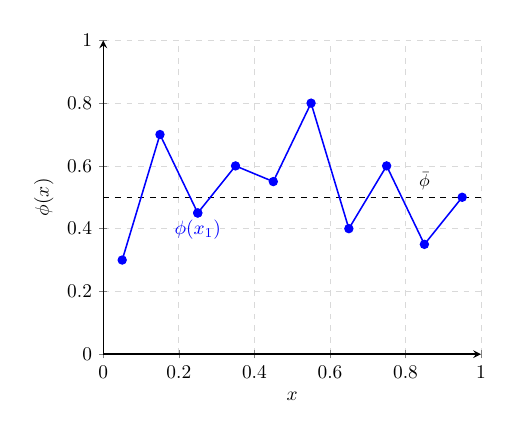
\begin{tikzpicture}[scale=0.7]
    \begin{axis}[
        ymin =0, ymax=1, 
        xmin=0, xmax=1, 
        xlabel = {$x$},
        ylabel = {$\phi(x)$},
        grid = both,                % griglia
        grid style = {dashed, gray!30},
        axis lines = left,          % assi più puliti
        thick, % linee più spesse
    ]

    
    \addplot[color=black,   domain=0:1, dashed]{0.5} node[pos=0.85, above, sloped] {\small $\bar{\phi}$};

    \addplot[
    mark=*,
    color=blue,
    thick, samples=2
] coordinates {
    (0.05,0.3)
    (0.15,0.7)
    (0.25,0.45)
    (0.35,0.6)
    (0.45,0.55)
    (0.55,0.8)
    (0.65,0.4)
    (0.75,0.6)
    (0.85,0.35)
    (0.95,0.5)
};

    \addplot[
    only marks,
    mark=*,
    mark size=2pt,
    color=blue
] coordinates {(0.25, 0.45)} node[below] {$\phi(x_1)$};
    
    \end{axis}
    \end{tikzpicture}

    \columnbreak

    La variabile si distribuisce intorno alla sua media $\bar{\phi}$ con una densità di probabilità che non dipende dalla x . Allora, anche se ho solo una realizzazione del processo, posso stimare

    \vspace{-0.65cm}
    
    \begin{align}
        <\phi(x_1)> &= \frac{1}{N}\sum_i^N\phi_i(x_1) \\
        &\simeq \frac{1}{N}\sum_i^N\phi(x_i) = \bar{\phi}
    \end{align}
    
\end{multicols}


Questa è una semplice visualizzazione monodimensionale delle medie che facciamo in cosmologia. \\

Considero ora la quantità $<\phi(x_1)\phi(x_2)>$. Se non vi è \emph{correlazione}, questo è uguale a $<\phi(x_1)><\phi(x_2)>$. Più in generale, scriviamo 
\begin{equation}
    <\phi(x_1)\phi(x_2)> = <\phi(x_1)><\phi(x_2)>\left[1 +  \xi(x_1 - x_2)\right]
\end{equation}

La funzione $\xi$ è detta \emph{funzione di autocovarianza}. Vedremo che la sua determinazione è di vitale importanza. \\
    
}

\ex{}{
    Consideriamo un volume $V$, contenente $N$ galassie. Indichiamo la sua densità numerica $\bar{n} = N/V$. Prendiamo ora due volumetti $dV_1, dV_2$, separati da una distanza $r$. Per definizione, si avrà $<dN_1> = \bar{n}dV_1$, $<dN_2> = \bar{n}dV_2$, e dunque $<dN_1dN_2> = \bar{n}^2dV_1dV_2[1 + \xi(r)]$.  \\

    Veniamo ora alla definizione di un importantissimo campo stocastico, il \emph{campo delle fluttuazioni}. 
    \begin{equation}
        \delta(\vec{x}) := \frac{\rho(\vec{x}) - \bar{\rho}}{\bar{\rho}}
    \end{equation}

    questo campo ha la comoda proprietà che $<\delta> = 0 \rightarrow \sigma^2 = <\delta^2>$. Si può definire per ogni campo stocastico, anche ad esempio per il numero di galassie: $\delta_g = \frac{n-\bar{n}}{n}$. \\

    Ora torniamo al problema precedente: 
    \begin{align}
        &<dN_1dN_2> = \bar{n}^2dV_1dV_2[1 + \xi(r)] \\
        & <n(x_1)n(x_2)> = \bar{n}^2[1  + \xi]\\
        & < (1+\delta(x_1))(1 + \delta(x_2))> = 1 + \xi \\
        & \quad 1 + \underbrace{<\delta(x_1)>}_{=0} + \underbrace{<\delta(x_2)>}_{=0} + <\delta(x_1)\delta(x_1 + r)> = 1 + \xi(r) \\
        & <\delta(x_1)\delta(x_1 + r)> = \xi(r)
    \end{align}

    Nel primo passaggio abbiamo diviso per $dV_1dV_2$, nel secondo abbiamo invertito la definizione della delta per trovare $\frac{n}{\bar{n}} = \delta + 1$, e nel terzo abbiamo svolto il prodotto. Osserviamo che il conto svela la grande importanza della funzione $\xi(r)$, anche perchè, valendo $<\delta> =0 \rightarrow \xi(0) = <\delta^2> = \sigma^2$. \\

    Veniamo alla discussione di come si può stimare $\xi(r)$ a partire dai dati sperimentali, ad esempio di una red-shift survey. \\

    Passando alle \emph{probabilità}, possiamo scrivere, sempre pensando all'esempio del cubo contenente $N$ galassie, 

    \begin{align}
        &\frac{<P_1P_2>}{<P_1>} = <P_2>(1+\xi)\\
        & P(2|1) = <P_2>(1+\xi) \\
        & P(2|1) = \frac{\bar{n}dV_2}{n_{tot}}(1+\xi)
    \end{align}

    Ora, immagino di pormi sulla galassia in $x_1$, e di contare quante gallassie sono presenti nel guscio sferico di raggio $r$ e di spessore $dr$: segue che l'elemento infinitesimo di volume sarà dato da $dV_2 = 41\pi r^2dr$, e dunque scriveremo

    \begin{equation}
        P(2|1) = \bar{n}4\pi r^2 dr(1+\xi(r))
    \end{equation}

    E definisco allora 
    \begin{equation}
        N^{GG} = 4\pi r^2 \bar{n}(1+\xi)
    \end{equation}

    Voglio estrapolare da questa equazione la funzione $\xi$, come posso fare? Osservo che posso prendere il mio numero $N$ di galassie, e disporle casualmente lungo il volume $V$, in modo tale che non vi sia correlazione. \\

    Allora chiaramente varrà 
    \begin{equation}
        1 + \xi (r) = \frac{N^{GG}(r)}{N^{RR}(r)}
    \end{equation}

    Che è nota come \emph{stima di Davis e Peebles}. La comodità di questa stima è che risolve un problema importante: se il guscio sferico esce dal mio volume, chiaramente su questo ci saranno meno galassie. Ma questo avviene sia per le galassie vere sia per le galassie random. Questo assicura che il rapporto dia una buona stima. \\

    Ci sono però altri due problemi che emergono nel caso dove le galassie vere non sono disposte in modo omogeneo, ma sono molto concentrate attorno al bordo del mio volume: allora molte volte il guscio conterrà meno galassie, perchè esce dal volume. Invece, il campione random disposto omogeneamente e come tale poche volte i suoi gusci escono dal volume. Il secondo problema è che se voglio avere informazioni sui claster molto densi, allora devo guardare $\xi(r)$ per $r$ molto piccolo, magari dell'ordine del $Mpc$. Da'altra parte, nel campione random nessuna coppia $N^{RR}$ sarà a distanze così piccole, così che di fatto queste distanze non riusciamo a campionarle. Questo effetto è noto come \emph{shot noise}. 
    
    Il problema si risolve nel seguente modo: 
    \begin{enumerate}
        \item 
        Si prende $N_{TOT}^R >> N_{TOT}^G$, così da avere sempre molte galassie random vicine, anche se la distribuzione è poco omogenea. Si tiene conto poi di questo rinormalizzando. 
        \item 
        Al posto di contare il numero di galassie random a partire da una galassia random, mi siedo sempre su una galassia vera, e confronto il numero di galassie random vicine rispetto a quelle reali. 
    \end{enumerate}

    Ora che ho applicato queste come correzioni, quale è la stima esatta? Il numero delle coppie di galassie è dato da 
    \begin{equation}
        N^{GG}_{TOT} = \frac{N_G(N_G -1)}{2}
    \end{equation}
    Mentre il numero di coppie galassie-random è semplicemente
    \begin{equation}
        N^{GR}_{TOT} = N_GN_R
    \end{equation}
        
    Dividendo ogni contributo per la sua normalizzazione, otteniamo che la stima è ora data da 
    \begin{tcolorbox}[colback=gray!15, colframe=black, boxrule=1pt]
    \begin{equation}
        \label{Peebles_davis}
        1 + \xi (r) = \frac{2N_R}{N_G -1}\frac{<N_{GG}(r)>}{<N_{GR}(r)>} 
    \end{equation}
    \end{tcolorbox}
}

Chiaramente, per $r$ grande, $\xi(r) \rightarrow 0$. D'altra parte, le fluttuazioni dei campi a grandi distanze sono di grande importanza per le osservazioni. Una possibile strategia è misurare la trasformata di Fourier del campo: questo viene molto utile anche perchè tipicamente le leggi teoriche vengono formulate in spazio di Fourier. 

\newpage

\begin{multicols}{2}
    \begin{samepage}
    \ex{}{
        Scomposizione in termini di fourier di un campo monodimensionale: 

        \vspace{0.5cm}
        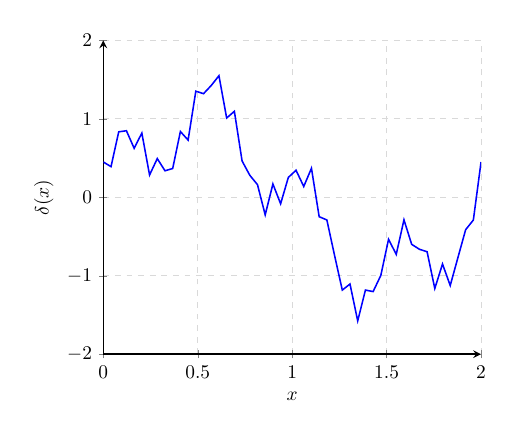
\begin{tikzpicture}[scale=0.7]
        \begin{axis}[
        ymin =-2, ymax=2, 
        xmin=0, xmax=2, 
        xlabel = {$x$},
        ylabel = {$\delta(x)$},
        grid = both,                % griglia
        grid style = {dashed, gray!30},
        axis lines = left,          % assi più puliti
        thick, % linee più spesse
    ]

    
    %\addplot[color=black,   domain=0:2, dashed]{sin(deg(pi*x))};

    \addplot[color=blue,   domain=0:2, samples=50]{sin(deg(pi*x)) + (0.5)*sin(deg(4*pi*x) + 30)+ (0.2)*cos(deg(20*pi*x))};

    %\addplot[color=black,   domain=0:2, dashed]{(0.6)*sin(deg(10*pi*x))};

    \end{axis}
    \end{tikzpicture}

    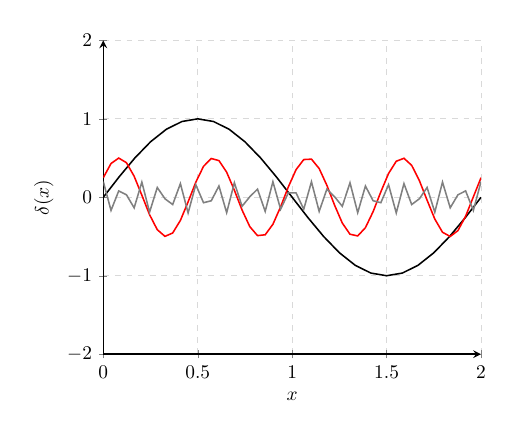
\begin{tikzpicture}[scale=0.7]
        \begin{axis}[
        ymin =-2, ymax=2, 
        xmin=0, xmax=2, 
        xlabel = {$x$},
        ylabel = {$\delta(x)$},
        grid = both,                % griglia
        grid style = {dashed, gray!30},
        axis lines = left,          % assi più puliti
        thick, % linee più spesse
    ]

    
    \addplot[color=black,   domain=0:2]{sin(deg(pi*x))};


    \addplot[color=red,   domain=0:2, samples=50]{(0.5)*sin(deg(4*pi*x) + 30)};
    \addplot[color=gray,   domain=0:2, samples=50]{(0.2)*cos(deg(20*pi*x))};

    \end{axis}
    \end{tikzpicture}   
    }
    \end{samepage}

    \columnbreak

    Scriveremo dunque 
    \begin{equation}
        \delta(\vec{r}) = \frac{1}{(2\pi)^3}\int d^3k \delta(\vec{k})e^{-i\vec{k}\cdot \vec{r}}
    \end{equation}

    Avendo definito 
    \begin{equation}
        \delta(\vec{k}) = \int d^3r\delta(\vec{r})e^{i\vec{k}\cdot\vec{r}}
    \end{equation}

    Ricordiamo una comoda rappresentazione della Delta di Dirac $\delta_D$ in termini di trasformata di Fourier: 
    \begin{equation}
        \delta_D(\vec{\mu}- \vec{r}) = \frac{1}{(2\pi)^3}\int d^3ke^{i\vec{k}(\vec{\mu}- \vec{r})}
    \end{equation}

    Considero due modi $\vec{k}_1, \vec{k}_2$, quanto vale $<\delta_{k_1}\delta^{*}_{k_2}> = ?$ \footnote{Chiaramente, dall'analisi di Fourier ci aspettiamo che queste siano ortogonali, così che siano sempre zero se $k_1 \neq k_2$. Nonostante ciò eseguiamo il calcolo per una coppia arbitraria, si tratta comunque di un calcolo istruttivo.} 
    \begin{equation}
        <\delta_{k_1}\delta^{*}_{k_2}> = <\int d^3r_1\delta(\vec{r}_1)e^{i\vec{k_1}\cdot\vec{r_1}}\int d^3r_2\delta(\vec{r}_2)e^{-i\vec{k_2}\cdot\vec{r}_2}>
    \end{equation}
\end{multicols}

Scrivendo $\vec{r} = \vec{r}_1 - \vec{r}_2$, posso scrivere 
\begin{equation}
     <\delta_{k_1}\delta^{*}_{k_2}> = <\int d^3r\delta(\vec{r} + \vec{r}_2)e^{i\vec{k_1}\cdot(\vec{r} + \vec{r_2})}\int d^3r_2\delta(\vec{r}_2)e^{-i\vec{k_2}\cdot\vec{r}_2}>
\end{equation}

Essendo fissi i limiti di integrazione, finchè non calcolo gli integrali posso spostare i termini a piacimento: 

\begin{equation}
    <\delta_{k_1}\delta^{*}_{k_2}> = <\int d^3r\delta(\vec{r} + \vec{r}_2)\delta(\vec{r}_2)e^{i\vec{k_1}\cdot\vec{r}} \underbrace{\int d^3r_2e^{i(\vec{k_1} - \vec{k_2})\cdot\vec{r}_2}}_{= (2\pi)^3\delta_D(\vec{k}_1 - \vec{k}_2)}>
\end{equation}

Gli unici cambi stocastici sono le $\delta$ così che l'op. di aspettazione agisce solo su di loro. D'altra parte, ci ricordiamo che $<\delta(x)\delta(x+r)> = \xi(r)$, coì da trovare infine 

\begin{equation}
    <\delta_{k_1}\delta^{*}_{k_2}> = \underbrace{\int d^3r\xi(r)e^{i\vec{k_1}\cdot\vec{r}}}_{:= P(k)}(2\pi)^3\delta_D(\vec{k_1} - \vec{k}_2)
\end{equation}

Abbiamo dfefinito la funzione $P(k)$, che è lo \emph{spettro di potenza}. L'eq. finale in termini di questa è detta \emph{definizione} dello spettro di potenza: 

\begin{tcolorbox}[colback=gray!15, colframe=black, boxrule=1pt]
\begin{equation}
    \label{definition_power_spectrum}
    <\delta_{k_1}\delta^{*}_{k_2} > = P(k)(2\pi)^3\delta_D(\vec{k}_1 - \vec{k}_2)
\end{equation}
\end{tcolorbox}

In pratica, però, come posso determinare la funzione $P(k)$ a partire dai dati sperimentali? Se immagino di prendere i miei dati da una red-shift survey, e immagino per il momento che il volume che ho a diposizione sia un cubo, allora posso fare una griglia del campo $\rho$, del campo $\delta$, e passarlo ad un algoritmo di fast-transform che mi restituisca la trasformata di Fourier. \\

Invece nel caso più probabile che il volume sia circa una fetta di torta, posso immaginare di immergerlo in un cubo, e scrivere $\delta_{torta} = \delta_{cubo}W(\vec{r})$. Allora, la trasformata di fourier sarà 
\begin{equation}
    \mathcal{F}(\delta_{torta}) = \mathcal{F}(\delta_{cubo}W) = \mathcal{F}(\delta_{cubo}) \times \mathcal{F}(W) = P(k) \times \underbrace{\mathcal{F}(W)}_{window \, function}  
\end{equation}

Tipicamente, quello che si osserva per la forma di $P(k)$ è un andamento del tipo 

\begin{multicols}{2}

    \begin{tikzpicture}[scale=0.7]
    \label{power_sprectrum}
    \begin{axis}[
        ymin =0, ymax=2, 
        xmin=0, xmax=1.5, 
        xlabel = {$logx$},
        ylabel = {$logP(k)$},
        grid = both,                % griglia
        grid style = {dashed, gray!30},
        axis lines = left,          % assi più puliti
        thick, % linee più spesse
    ]

    \addplot[color=black,   domain=0:0.6]{-1.5*x*(x-1.5)*exp(-(x-1)^2)*exp(-(1-x)/2)};
    \addplot[color=black,   domain=0.6:1, dashed]{-1.5*x*(x-1.5)*exp(-(x-1)^2)*exp(-(1-x)/2)};
    \addplot[color=black,   domain=1:2]{-1.5*x*(x-1.5)*exp(-(x-1)^2)*exp(-(1-x)/2)};

    \begin{pgfonlayer}{background}
            \fill[blue!10]  (axis cs:0,0)   rectangle (axis cs:0.6,2);
            \fill[green!10] (axis cs:1,0) rectangle (axis cs:1.5,2);
        \end{pgfonlayer}


        
        % --- Note sul grafico ---
        \node at (axis cs:0.25, 1.1) {\small CMB};
        \node at (axis cs:1.2,1.6) {\small red-shift};
        \node at (axis cs:1.2,1.5) {\small surveys};
    
    \end{axis}   
    \end{tikzpicture}

    \columnbreak

    grafico in scala log-log. Nelle scale osservate dai red-shift surveys, l'andamento è descrescente con legge $\simeq k^{-2}$. Se uniamo questi alle stime date dal CMB, possiamo ottenere informazioni su $k$ più piccoli, dove si ha circa $\simeq k^{-1}$. 
\end{multicols}

Ora, noi sappiamo che, dall'ipotesi di ergodicità e anche dall'ipotesi di isotropia, che $\xi(\vec{r}) = \xi(r = |\vec{r}|)$. Chiaramente questo implica che anche $P=P(k = |\vec{k}|)$. Possiamo allora scrivere la sua definizione in termini più semplici? Questa era data da 

\begin{equation}
    P(\vec{k}) = \int d^3r\xi(r)e^{i\vec{k_1}\cdot\vec{r}}
\end{equation}

Dato che $\xi$ è una funzione del modulo di $\vec{r}$ la scelta più naturale è passare ad un integrale in coordinate sferiche. Scelgo accuratamente l'asse $z \, || \, \vec{k}$, così che valga $\vec{k}\cdot \vec{r} = kr\cos{\theta}$, e che io possa scrivere 

\begin{equation}
    P(k) = \int_0^{2\pi}d\varphi\int_0^{+\infty}dr\int_0^\pi d\theta \sin{\theta}e^{ikr\cos{\theta}}  r^2 \xi(r)
\end{equation}

A questo punto conviene effettuare la sostituzione $x = \cos{\theta}$, così che $dx = -\sin{\theta}d\theta$, e dunque che valga 

\begin{align}
    P(k) &= 2\pi \int_0^{+\infty}dr r^2\xi(r)\int_{-1}^1dx e^{ikrx} \\
    P(k)&= 2\pi \int_0^{+\infty}dr r^2\xi(r)\frac{e^{ikrx}}{ikr}\biggr|^1_{-1} \\
    P(k )&= \int_0^{+\infty}dr 4\pi r^2\xi(r)\frac{\sin{kr}}{kr} 
\end{align}

Che è proprio la formula che stavamo cercando. In base a questa, che andamento avrà $P(k)$ se prendiamo una forma nota di $\xi(r)$, ad esempio le prime misure di Peebles, $\xi(r) \simeq r^{-\gamma}, \, \gamma \simeq 1.8 \quad r\in (0.1, 1) Mpch^{-1}$?

Sostituiamo l'espressione di $\xi$ nella formula, e facciamo la sostituzione $x = kR$. Allora ottengo 
\begin{equation}
    P(k) = \int_0^{+\infty} \frac{x^{-\gamma}}{k^{-\gamma}}\frac{\sin{x}}{x}4\pi\frac{x^2}{k^2}\frac{dx}{k}
\end{equation}

Ci accorgiamo che se l'integrale in $x$ converge, allora la $P(k) \propto k^{\gamma -3}$. Dunque per le misure di Peebles, $P(k)\propto k^{-1.2}$. \\

Vedremo nel dettaglio più in avanti come l'evoluzione temporale giustifichi la forma dello spettro di potenza, della figura \ref{power_sprectrum}. Anticipiamo il ragionamento: consideriamo ora un campo delle fluttuazioni, considerando anche la dipendenza temporale $\delta = \delta(\vec{x}, t)$. Ci sono due possibiltà: 
\begin{enumerate}
    \item 
    Le fluttuazioni sono piccole. Allora la decomposizione in serie di Fourier può considerarsi in ottima approssimazione esatta, e posso linearizzare le eq. del moto per il campo $\delta$. Così, $\delta(\vec{x}, t ) \rightarrow \sum \delta_k$, e siccome le eq. sono lineari, ciascun $\delta_k$ evolverà nel tempo allo stesso modo. Questa approssimazione vale in due situazioni: l'universo primordiale, e l'universo attuale a scale molto grandi. 
    \item 
    Le fluttuazioni non sono piccole. Questo avviene dopo l'espandersi dell'universo ed a scale dove la gravità è rilevante. In questo caso, i $\delta_k$ evolvono indipendentemente. 
\end{enumerate}

Questo spiega una evoluzione temporale come illustrata in figura: 

\begin{multicols}{2}
    \begin{tikzpicture}[scale=0.7]
    \begin{axis}[
        ymin =0, ymax=2, 
        xmin=0, xmax=1.5, 
        xlabel = {$logk$},
        ylabel = {$logP(k)$},
        grid = both,                % griglia
        grid style = {dashed, gray!30},
        axis lines = left,          % assi più puliti
        thick, % linee più spesse
    ]

    \pgfmathdeclarefunction{f}{1}{
        \pgfmathparse{-1.5*#1*(#1-1.5)*exp(-(#1-1)^2)*exp(-(1-#1)/2)}
    }

    \addplot[color=black,   domain=0:1.5]{-1.5*x*(x-1.5)*exp(-(x-1)^2)*exp(-(1-x)/2)};

    %\addplot[color=black,   domain=0:1.5]{f(x)};

    \addplot[color=black, domain=0:1, dashed]
        {-1.5*x*(x-1.5)*exp(-(x-1)^2)*exp(-(1-x)/2) + 0.3};

    \addplot[color=black, domain=1:1.5, dashed]
        {-1.5*x*(x-1.5)*exp(-(x-1)^2)*exp(-(1-x)/2) + 0.3 - 0.4*(x-1)};


    \begin{pgfonlayer}{background}
            \fill[blue!10]  (axis cs:0,0)   rectangle (axis cs:1,2);
            \fill[green!10] (axis cs:1,0) rectangle (axis cs:1.5,2);
        \end{pgfonlayer}


        
        % --- Note sul grafico ---
        \node at (axis cs:0.45, 1.3) {\small grandi scale};
        \node at (axis cs:0.45, 1.2) {\small piccole oscillazioni};
        \node at (axis cs:1.25,1.6) {\small piccole scale};
        \node at (axis cs:1.25,1.5) {\small regime non};
        \node at (axis cs:1.25,1.4) {\small lineare};

        \draw[->, thick, purple] (axis cs:0.4,{f(0.4)}) -- (axis cs:0.4,{f(0.4)+0.3});

        \draw[->, thick, purple] (axis cs:0.8,{f(0.8)}) -- (axis cs:0.8,{f(0.8)+0.3});
    
    \end{axis}   
    \end{tikzpicture}

    \columnbreak    

    A scale grandi, si mantiene una forma che corrisponde alla "firma" dell'universo primordiale. Con l'avanzare dell'espansione, la regione non lineare di scale piccole tende a modificare sempre di più lo spettro. 
\end{multicols}


Vediamo dei calcoli che ci permettono di meglio comprendere cosa ci sta dicendo la funzione $P(k)$ e perchè molte volte sia comodo utilizzare una sua variante $\Delta_k^2$, dal significato fisico più manifesto. \\

Ricordando la proprietà di un campo stocastico a media nulla $\xi(0) = \sigma^2$, scrivendo $\xi$ in trasformata e dunque in termini di spettro di potenza, si ottiene

\begin{equation}
    \sigma^2 = \frac{1}{(2\pi)^3}\int d^3k P(\vec{k})e^{-i\vec{k}\cdot \vec{r}}\biggr|_{\vec{r}=0} = \frac{1}{(2\pi)^3}\int d^3kP(\vec{k})
\end{equation}

se $P=P(k)$, cioè se ho un processo isotropo, 
\begin{equation}
    \sigma^2 = \int \frac{P(k)}{(2\pi)^3}(4\pi k^2 )dk = \int \frac{P(k)}{(2\pi)^3}(4\pi k^3 )d(\ln{k}) 
\end{equation}

L'ultima uguaglianza è comoda perchè spesso considereremo grafici in scala log-log. Definiamo allora 
\begin{equation}
    \Delta_k^2 = \frac{k^3}{2\pi^2}P(k)
\end{equation}

Che ci dice proprio la varianza ad un dato vettore d'onda $k$. Osserviamo che, se prendiamo la forma di $\Delta_k^2$ data la $P(k)$ della figura \ref{power_sprectrum}, otteniamo una funzione monotona crescente, come ci aspettavamo. \\

A volte, noi vorremmo considerare un campo stocastico di fluttuazioni \emph{filtrato}. Questo vuol dire che considereremo, ad esempio, dei campi del tipo 
\begin{equation}
    \delta_R(\vec{x}) = \int \delta(\vec{x}- \vec{y})W(\vec{y}) d^3y
\end{equation}

Dove la funzione $W$ è il filtro (e.g. $\theta$ di heaviside, gaussiana, ecc.). Trattandosi di una convoluzione, è conveniente passare allo spazio di fourier: 

\begin{equation}
    \delta_R(\vec{k}) = \delta_R(\vec{k})W_R(\vec{k})
\end{equation}

Dove abbiamo sottointeso (con un abuso di notazione) $W_R(\vec{k}) = \mathcal{F}(W_R(\vec{x}))$. Questo rivela la comodità di un filtro gaussiano, che rimane gaussiano anche sotto trasf. di fourier. 

Se considero campi filtrati, vediamo che possiamo considerare il campo delle flutuazione della densità come il campo di fluttuazioni della massa (basta moltiplicare per il volume):
\begin{equation}
    \delta_R(\vec {x} ) = \frac{\rho(\vec{x})- \bar{\rho}}{\bar{\rho}} = \frac{M_r(\vec{x}) - \bar{M_R}}{\bar{M_R}} = \frac{\Delta M_R(\vec{x})}{\bar{M_R}} = \delta M_R 
\end{equation}

Chiaramente, 
\begin{equation}
    \Delta M_R(\vec{x}) = \bar{\rho}V \delta_R(x) = \bar{\rho}V\int \delta(\vec{x} - \vec{y})W_R(\vec{y})d^3y
\end{equation}

ed applicando la trasformata di Fourier, intendendo sempre con il solito abuso di notazione $\Delta M_R(\vec{k}) = \mathcal{F}(\Delta M_R(\vec{x}))$, scriveremo

\begin{equation}
    \Delta M_R(\vec{k}) = \bar{\rho}V\delta(\vec{k})W_R(\vec{k})
\end{equation}

Chiaramente questo indica che il campo delle fluttuazioni della massa in trasformata di fourier diventa 
\begin{equation}
    \delta M_r(\vec{k}) = \frac{\Delta M_R(\vec{k})}{\bar{M_R}} = \frac{\bar{\rho}V\delta(\vec{k})W_R(\vec{k})}{\bar{\rho}V} = \delta(\vec{k})W_R(\vec{k})
\end{equation}

Riscrivendo $\delta M_R(\vec{x})$ in antitrasformata di Fourier, scriveremo allora
\begin{align}
    \delta M_R(\vec{x}) &= \mathcal{F^{-1}}(\delta M_R(\vec{k})) = \frac{1}{(2\pi)^3}\int d^3k \delta M_R(\vec{k}) e^{-i \vec{k}\cdot \vec{r}} \\
    &= \frac{1}{(2\pi)^3}\int d^3k \delta(\vec{k})W_R(\vec{k})e^{-i\vec{k}\cdot \vec{r}}
\end{align}

Ora, la varianza sarà data da $\sigma^2 = <\delta M_R^2>$, e ricordando l'eq. \ref{definition_power_spectrum}, otteniamo
\begin{equation}
    <\delta M_r^2> = \frac{1}{(2\pi)^3}\int d^3k P(\vec{k})|W_R(\vec{k})|^2
\end{equation}

Determiniamo dunque la varianza calcolando l'integrale se vale $P(k) = Ak^n$, e se il filtro è gaussiano. \\

Per prima cosa svolgiamo l'integrale per parti: 
\begin{align}
    <\delta M_r^2> &= \frac{1}{(2\pi)^3}\int dk4\pi k^2 Ak^n|W_R(k)|^2 \\
    &\propto \left[k^{n+3}|W_R(k)|^2\right]_0^{+\infty} - \int_0^{+\infty}k^{n+3}\left( \frac{d}{dk}|W_R(k)|^2\right) dk
\end{align}

Ora, la prima parte dei contributi al contorno fa zero, perchè per $k=0$ supponiamo che il filtro non faccia niente di strano (d'altra parte perchè dovrebbe, è solo un filtro), e quando andiamo all'infinito se il filtro è buono andrà a $0$ molto più velocemente di una legge di potenza. Queste sono considerazioni che valgono per qualunque buona scelta di filtro, e in particolare nel nostro caso di filtro gaussiano. Calcoliamo quindi la derivata del modulo della funzione finestra: Se $W_R(x) = \frac{1}{\sqrt{2}R}e^{-\frac{x^2}{2R}}$, allora vale $W_R(k) = \mathcal{F}(W_R(x)) = e^{-\frac{k^2R^2}{2}}$, ed in particolare 

\begin{equation}
    \frac{d}{dk}|W_R(k)|^2 = -2R^2ke^{-k^2R^2z}
\end{equation}

Così che troveremo
\begin{equation}
    \sigma_M^2 \propto \int_0^{+\infty} 2R^2k^{n+4}e^{-k^2R^2}dk \xrightarrow{x = kR} \frac{2}{R^{n+3}}\int_0^{+\infty}x^{n+4}e^{-x^2}dx \propto R^{-(n+3)} 
\end{equation}

Ricordandosi anche che $R \propto M^{1/3}$, otteniamo un legame fra la varianza di massa e la massa, 
\begin{equation}
    \sigma_M^2 \propto  M^{-\frac{3+n}{3}}
\end{equation}


Fino ad adesso abbiamo assunto che il campo delle fluttuazioni delle galassie fosse sostanzialmente la stessa cosa che il campo delle fluttuazioni della densità di materia. Verso la fine degli anni '80, i cosmologi cominciarono a dubitare di questo. Infatti, se questo fosse vero, allora la funzione di correlazione $\xi$ dovrebbe essere la stessa indipendentemente se la misuro a partire da una galassia oppure da un'altra. Quello che si osservò invece fu: 

\begin{enumerate}
    \item 
    il confronto di $\xi$ fra galassie ellittiche e galassie a spirale, rappresentato in figura:  

    \vspace{0.5cm}
    \begin{multicols}{2}
        
    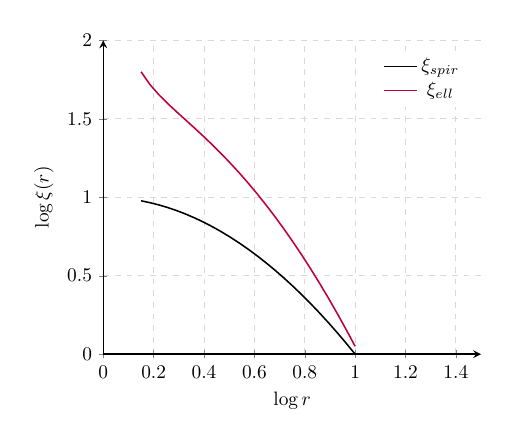
\begin{tikzpicture}[scale=0.7]
        \begin{axis}[
    ymin=0, ymax=2,
    xmin=0, xmax=1.5,
    xlabel={$ \log r $},
    ylabel={$ \log \xi(r) $},
    grid=both,
    grid style={dashed, gray!30},
    axis lines=left,
    thick,
    legend style={
        at={(0.97,0.97)},          % posizione in coordinate relative (1,1) = angolo in alto a destra
        anchor=north east,         % ancora il punto in alto a destra
        draw=none,                 % nessun bordo
        %font=\small,
        %fill=none,                 % sfondo trasparente
    },
]
    % Linea semplice
    \addplot[color=black, domain = 0.15:1]{1-x^2};
    \addlegendentry{$\xi_{spir}$}
    
    % Linea più complessa ottimizzata
    \addplot[color=purple, domain=0.15:1]{1.5*(1-x^2) + 0.05/x};
    \addlegendentry{$\xi_{ell}$}
    \end{axis}
    \end{tikzpicture}


    \columnbreak
    Questo da noi oggi e attribuito alla diversa astrofisica che governa questi oggetti per $r$ piccolo, mentre la differenza ad $r$ grande si spiega per la massa più grande che caratterizza questi oggetti, come spiegato dopo.

    \end{multicols}


    \item 
    A livello teorico, dovrebbe essere equivalente calcolare $\xi$ per le galassie, e $\xi$ per i grandi ammassi di galassie. Avendo a disposizione grandi cataloghi (e.g. Abell) degli ammassi di galassie, si fece il calcolo nel secondo caso, e si ottenne: 
    \begin{multicols}{2}
        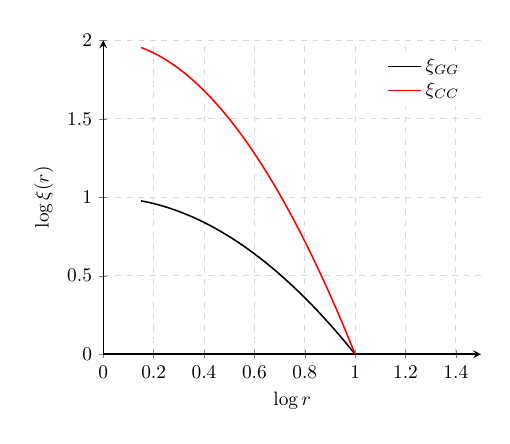
\begin{tikzpicture}[scale=0.7]
        \begin{axis}[
    ymin=0, ymax=2,
    xmin=0, xmax=1.5,
    xlabel={$ \log r $},
    ylabel={$ \log \xi(r) $},
    grid=both,
    grid style={dashed, gray!30},
    axis lines=left,
    thick,
    legend style={
        at={(0.97,0.97)},          % posizione in coordinate relative (1,1) = angolo in alto a destra
        anchor=north east,         % ancora il punto in alto a destra
        draw=none,                 % nessun bordo
        %font=\small,
        %fill=none,                 % sfondo trasparente
    },
]
    % Linea semplice
    \addplot[color=black, domain = 0.15:1]{1-x^2};
    \addlegendentry{$\xi_{GG}$}
    
    % Linea più complessa ottimizzata
    \addplot[color=red, domain = 0.15:1]{2*(1-x^2)};
    \addlegendentry{$\xi_{CC}$}
    \end{axis}
    \end{tikzpicture}

    \columnbreak

    Come nel caso di prima, a grandi $r$ sembra esserci un fattore moltiplicativo (di circa 5).fra il conteggio delle galassie-galassie ed il conteggio cluster-cluster. 
    \end{multicols}

    \end{enumerate}

    Questi indizi portarono i cosmologi del tempo a pensare che $\delta_g$ fosse una funzione del campo di fluttuazioni di densità $\delta$, che in prima approssimazione poteva essere preso lineare: 

    \begin{equation}
        \delta_G = \delta_G(\delta) \simeq b_L \delta
    \end{equation}

    Il coefficiente lineare $b_L$ è detto \emph{fattore di bias}. Questo poi si trasmette alle funzioni di correlazioni $\xi$, perchè $\xi_{gg} = b_L^2\xi_\rho$. Ma a cosa è dovuto questo fattore di bias? In realtà, con sorpresa si scoprì poco dopo che si trattava di un mero effetto statistico: 

    Prendiamo infatti una realizzazione di un processo stocastico (per comodità unidimensionale), e supponiamo di filtrare solo gli elementi al di sopra di una certa soglia: 

    \begin{multicols}{2}

    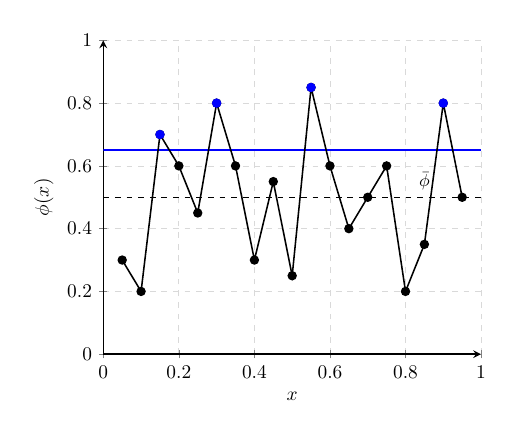
\begin{tikzpicture}[scale=0.7]
    \begin{axis}[
        ymin =0, ymax=1, 
        xmin=0, xmax=1, 
        xlabel = {$x$},
        ylabel = {$\phi(x)$},
        grid = both,                % griglia
        grid style = {dashed, gray!30},
        axis lines = left,          % assi più puliti
        thick, % linee più spesse
    ]

    
    \addplot[color=black,   domain=0:1, dashed, samples=2]{0.5} node[pos=0.85, above, sloped] {\small $\bar{\phi}$};
    \addplot[color=blue,   domain=0:1]{0.65};

    \addplot[
    mark=*,
    color=black,
    thick, 
    samples=2
] coordinates {
    (0.05,0.3)
    (0.10,0.2)
    (0.15,0.7)
    (0.20,0.6)
    (0.25,0.45)
    (0.30,0.8)
    (0.35,0.6)
    (0.40,0.3)
    (0.45,0.55)
    (0.50,0.25)
    (0.55,0.85)
    (0.60,0.6)
    (0.65,0.4)
    (0.70,0.5)
    (0.75,0.6)
    (0.80,0.2)
    (0.85,0.35)
    (0.90,0.8)
    (0.95,0.5)
};

    \addplot[
    only marks,
    mark=*,
    mark size=2pt,
    color=blue
] coordinates {(0.15, 0.7)};

    \addplot[
    only marks,
    mark=*,
    mark size=2pt,
    color=blue
] coordinates {(0.55, 0.85)};

    \addplot[
    only marks,
    mark=*,
    mark size=2pt,
    color=blue
] coordinates {(0.90, 0.8)};

    \addplot[
    only marks,
    mark=*,
    mark size=2pt,
    color=blue
] coordinates {(0.30, 0.8)};
    
    \end{axis}
    \end{tikzpicture}

    \columnbreak

    In riferimento alla figura, questo vuol dire considerare solo gli elementi colorati in blu. Di fatto, se vado a fare una statistica su questi punti, la loro funzione di correlazione viene scalata rispetto a quella di tutti i punti, con una legge del tipo (se i punti sono distribuiti gaussianamente)

    \vspace{-0.5cm}
    \begin{equation}
        \xi_{\nu, R} = \exp{\left(\frac{\nu^2}{\sigma_R^2}\xi_R(r) \right)} \simeq \underbrace{\frac{\nu^2}{\sigma_R^2}}_{=b_L^2}\xi(r)
    \end{equation}
    \end{multicols}

\newpage

\chapter{Evoluzione delle perturbazioni}

\section{La teoria di Jeans}

Ci poniamo ora la questione di determinare la dipendenza temporale di $\delta(\vec{x}, t)$. Per farlo, useremo la teoria di Jeans, ovvero prenderemo le eq. per la dinamica di un fluido sotto certe ragionevoli assunzioni, e le linearizzeremo, facendo l'assunzione di piccole perturbazioni. In particolare, assumeremo un fluido autogravitante che sia 
\begin{enumerate}
    \item \emph{autogravitante}, questo vuol dire considerare un campo gravitazionale che sia dato dall'eq. di Poisson
    \item \emph{non relativistico}, ovvero con $v << c$. 
    \item a scale molto minori dell'orizzonte cosmologico, ovvero minori di $ct_0 \simeq \frac{c}{H_0}$. 
    \item a singola componente, ovvero ad esempio se il fluido è costituito da materia e radiazione, queste siano perfettamente accopiate (come prima della riconbinazione). 
\end{enumerate}

Sotto queste ipotesi, i campi rilevanti che entreranno nelle equazioni sono $\rho(\vec{x}, t), \vec{v}(\vec{x}, t), p(\vec{x}, t), \phi(\vec{x}, t)$. Le forze in gioco saranno date solamente dai gradienti di pressione e dalla gravità, così che le equazioni sono: \\

L'equazione di continuità, che discende direttamente dalla conservazione della massa
\begin{equation}
    \frac{\partial \rho}{\partial t} + \vec{\nabla} \cdot (\rho\vec{v}) = 0
\end{equation}

Le eq. del moto dette eq. di Eulero:
\begin{equation}
    \frac{\partial \vec{v}}{\partial t} + (\vec{v}\cdot\vec{\nabla})\vec{v} = -\frac{\vec{\nabla} p}{\rho} - \vec{\nabla}\phi
\end{equation}

E infine l'eq. di Poisson: 
\begin{equation}
    \nabla^2\phi = 4\pi G \rho
\end{equation}

Poichè siamo interessati alle perturbazioni, scriveremo le quantità come le quantità all'equilibrio più una piccola variazione: 

\[\begin{cases}
    \rho = \rho_0(1+\delta) \\
    \vec{v} = \vec{v}_0 + \vec{v}^{'}\\
    p = p_0 + p^{'}\\
    \phi = \phi_0 + \phi^{'}
\end{cases}\]

Dove ad esempio notiamo che $\rho_0 = \rho_0(t)$ perchè si tratta della densità di backround. \\
Sostituendo queste espressioni nelle equazioni precedenti, e mantenendo solo i termini del primo ordine, si ottiene la loro versione linearizzata. A titolo di esempio, vediamo il semplice calcolo nel caso dell'eq. di continuità: 

\begin{align}
    &\frac{\partial}{\partial t}\left(\rho_0(1+\delta)\right) + \vec{\nabla}\cdot [\rho_0(1+\delta)(\vec{u}_o + \vec{u}')] =0 \\
    & \frac{\partial \rho_0}{\partial t}(1+\delta) + \rho_0 \frac{\partial \delta}{\partial t}\rho_0 + \rho_0(\vec{\nabla}\delta \cdot \vec{u}_0 + (1+\delta)\vec{\nabla}\cdot(\vec{u}_0 + \vec{u}')) =0
\end{align}

Ora riconosco il termine imperturbato e divido per \(\rho_0\): 

\begin{align}
    &\frac{\partial \delta}{\partial t} + \vec{u}_0 \cdot \vec{\nabla}\delta + (1+\delta)\vec{\nabla}\cdot \vec{u}' =0 \\
    & \frac{d\delta}{dt} = -\vec{\nabla}\cdot \vec{u}'
\end{align}


Procedendo con la stessa ricetta, otteniamo l'eq. di Eulero linearizzata
\begin{equation}
    \frac{d\vec{v}^{'}}{dt} + (\vec{v}^{'}\cdot \vec{\nabla})\vec{v}_0 = -\frac{\vec{\nabla}p^{'}}{\rho_0} - \vec{\nabla}\phi^{'}
\end{equation}

e l'eq. di Poisson linearizzata
\begin{equation}
    \nabla^2\phi = 4\pi G\rho_0 \delta
\end{equation}

Ora, queste equazioni vanno bene ma sono ancora scritte nelle coordinate fisiche. Vorremmo invece scriverle in termini di coordinate \emph{comoventi}. Sappiamo che le due sono legate dalla relazione 
\begin{equation}
    \vec{x}(t) = a(r)\vec{r}(t)
\end{equation}
Dove $\vec{r}$ dipende ancora dal tempo perchè questa può variare per fattori diversi dalla espansione. Derivando, troviamo la trasformazione per le velocità: 
\begin{equation}
    \frac{d\vec{x}}{dt} = a\frac{d\vec{r}}{dt} + \dot{a}\vec{r} = a\frac{d\vec{r}}{dt} + \frac{\dot{a}}{a}\vec{x} 
\end{equation}

Definendo le velocità peculiari $\vec{u} = \frac{d\vec{r}}{dt}$, e ricordando il parametro di Hubble $H = (\dot{a}/a)$, scriviamo dunque 
\begin{equation}
    \frac{d\vec{x}}{dt} = H\vec{x} + a\vec{u}
\end{equation}

Confrontando questa con l'espressione $\vec{v} = \vec{v}_0 + \vec{v}^{'}$, possiamo identificare 
\[\begin{cases}
    \vec{v}_0 = H\vec{x} \\
    \vec{v}^{'} = a\vec{u}
\end{cases}\]

L'unica cosa che ci resta da comprendere come si trasformano sono i gradienti. Ma questi in realtà sono molto semplici, perchè
\begin{equation}
    \vec{\nabla} = \left(\frac{\partial}{\partial x}, \frac{\partial}{\partial y}, \frac{\partial}{\partial z} \right) = \frac{1}{a}\left(\frac{\partial}{\partial r_x}, \frac{\partial}{\partial r_y}, \frac{\partial}{\partial r_z} \right) = \frac{1}{a}\vec{\nabla}_r
\end{equation}

Sostituendo, troviamo le equazioni: 
\begin{equation}
    \dot{\delta} = -(\vec{\nabla}_r \cdot \vec{u})
\end{equation}
\begin{equation}
    \frac{d\vec{u}}{dt} + 2H\vec{u} = -\frac{1}{a^2}\left (\frac{\vec{\nabla}_r p}{\rho_0} + \vec{\nabla}\phi\right)
\end{equation}
\begin{equation}
    \nabla^2_r\phi = 4\pi G \rho_0 \delta a^2
\end{equation}


Ora, vorremmo compattare le 3 equazioni in una sola. Per risolverla, dovremmo anche esplicitare il rapporto fra $p, \rho$. Per farlo assumiamo un fluido isentrpico, allora vale 
\begin{equation}
    \delta p = \frac{\partial p}{\partial \rho}d\rho = c_s^2 d\rho
\end{equation}
Così che la perturbazione della pressione diventi
\begin{equation}
    p^{'} = c_s^2\delta\rho_0
\end{equation}

Al fine di unire le equazioni, deriviamo la prima rispetto al tempo: 
\begin{equation}
    \ddot{\delta} = -(\vec{\nabla}_r \cdot \vec{\dot{u}})
\end{equation}

Applicando poi la divergenza alla seconda equazione, ricordandiomi che $\nabla^2 p^{'} = c_s^2\rho_0 \nabla^2\delta$, scriverò

\begin{equation}
    \ddot{\delta} + 2H\dot{\delta} = \left(4\pi G \rho_0 + \frac{c_s^2}{a^2}\nabla^2_r\right)\delta
\end{equation}

Abbiamo dunque trovato un'equazione differenziale alle derivate parziali lineare in $\delta$. Per studiarne le soluzioni, passiamo in spazio di Fourier, dove diventa un'equazione ordinaria $\delta \rightarrow \int \delta_k e^{-ikr}dk$, 

\begin{tcolorbox}[colback=gray!15, colframe=black, boxrule=1pt]
\begin{equation}
    \label{linear_growth_equation}
    \ddot{\delta}_k + 2H\dot{\delta}_k = \left(4\pi G \rho_0 - \frac{c_s^2k^2}{a^2}\right)\delta_k
\end{equation}
\end{tcolorbox}

Questa è l'equazione di crescita lineare delle perturbazioni. Osserviamo che il termine all'interno delle parentesi indica il bilanciamento tra i gradienti di pressione e la gravità. Potremmo definire la lunghezza d'onda dove l'intera parentesi si annulla, data da 

\begin{equation}
    \frac{4\pi^2}{\lambda_j} = \frac{4\pi G\rho_0}{c_s^2} \rightarrow \lambda_j = c_s\sqrt{\frac{\pi}{G\rho_0}}
\end{equation}

La lunghezza $\lambda_j$ è detta \emph{lunghezza di Jeans}. Questa è importante per la dinamica di $\delta_k$, perchè se $\lambda > \lambda_j$, allora il fluido collassa, se $\lambda < \lambda_j$, allora le perturbazioni hanno un comportamento oscillante. \\

Come interpetiamo invece il termine $2H\dot{\delta}_k$? Questo è un fattore interessante, perchè se osserviamo l'eq. \ref{linear_growth_equation}, e notiamo la somiglianza con l'eq. per un oscillatore armonico smorzato, questo è proprio il termine di viscosità. Di fatto, poichè si tratta di un fattore \emph{positivo}, questo fattore tiene conto che se l'universo è in espansione, un eventuale collasso deve anche vincere l'espansione stessa. Per questo fatto, il fattore è anche detto \emph{expansional drag}. \\

\section{Crescita delle fluttuazioni nell'era della materia}

Cominciamo allora a studiare delle soluzioni dell'eq. \ref{linear_growth_equation}. Prendiamo una situazione dove $\lambda >> \lambda_j$, così che l'eq. sia data da 
\begin{equation}
    \ddot{\delta}_k + 2H\dot{\delta}_k = 4\pi G \bar{\rho}\delta_k
\end{equation}

Per risolverla devo specificare da cosa sono dati $H=H(t)$, $\bar{\rho}= \bar{\rho}(t)$. Questo dipende dalle condizioni fisiche. Ad esempio assumiamo che l'universo sia dominato dalla materia, e che valga $a <<1$. Questo perchè se scriviamo la 1° Friedmann, \ref{first_friedman}, 
\begin{equation}
    H^2 = H_0^2(\Omega_{m0}a^{-3}+ \Omega_{\gamma 0}a^{-4} + \Omega_{\Lambda} + \Omega_ka^{-2}) \simeq H_0^2\Omega_{m0}a^{-3}
\end{equation}

E dunque questa può essere facilmente integrata, 
\begin{equation}
    a(t) = \left(\frac{3}{2}H_0 \right)^{2/3}t^{2/3} = \alpha t^{2/3}
\end{equation}
Se la deriviamo otteniamo
\begin{equation}
    \dot{a}(t) = \frac{2}{3}\alpha t^{-1/3} \rightarrow H(t) = \frac{\dot{a}}{a} = \frac{2}{3}t^{-1}
\end{equation}

Consideriamo ora $\bar{\rho}(t)$: sappiamo che, nell'era della materia
\begin{equation}
    \bar{\rho}(t) = \rho_0a^{-3} = \rho_0\left(\frac{3H_0}{2} \right)^{-2}t^{-2}
\end{equation}

Dove nella seconda uguaglianza abbiamo esplicitato $a=a(t)$. D'altra parte, $\rho_0$ è la densità di oggi, ed essendo in un universo di $\mathcal{E}dS$, chiaramente deve valere $\rho_o = \rho_{crit} = \frac{3H_0^2}{8\pi G}$, così da ottenere 
\begin{equation}
    \bar{\rho}(t) = \frac{t^{-2}}{6\pi G} 
\end{equation}

Così che l'equazione di crescita lineare diventa: 
\begin{equation}
    \ddot{\delta} + \frac{4}{3}\dot{\delta} t^{-1} -\frac{2}{3}t^{-2}\delta =0
\end{equation}

i coefficenti $t^{-1}, t^{-2}$ suggeriscono di cercare delle soluzioni del tipo $\delta(t) = At^n$. Sostituendo, otteniamo che: 

\begin{equation}
    t^{n-2}\left(n^2 - n +\frac{4}{3}n - \frac{2}{3}\right) = 0 \quad \forall t
\end{equation}

Risolvendo l'eq. algebrica di secondo grado otteniamo $n_1 = \frac{2}{3}, n_2 = -1$. \\

concludiamo che la soluzione più generale sarà data da 
\begin{equation}
    \delta(t) = c_1\delta^{+}(t) + c_2\delta^{-}(t)
\end{equation}

dove
\[\begin{cases}
    \delta^{+}(t) = t^{2/3} \\ \delta^{-}(t) = t^{-1}
\end{cases}\]

Osservando che la soluzione $\delta^{-}$ è una soluzione transiente che dopo un certo tempo può essere trascurata, troviamo che $\delta(t)\propto t^{2/3}$, così come $a(t) \propto t^{2/3}$. Concludiamo dunque che, in $\mathcal{E}dS$, vale $\delta(a) \propto a$. \\

Cosa succede se invece l'universo non è dominato dalla materia? Possiamo vederlo in un caso estremo, l'\emph{universo vuoto} di Milne, dove si prende il limite $\rho \rightarrow 0$. Questo tipo di universo fu studiato verso la metà del secolo scorso, così che $\Omega_\Lambda = 0$. D'altra parte, ci mettiamo con $a$ sufficientemente grande così che anche $\Omega_\gamma$ sia trascurabile. Gli unici contributi sono dunque $\Omega_m, \Omega_k$ di cui il primo lo prendo infinitesimo. In questo limite, la prima equazione di Friedmann \ref{first_friedman} diventa: 

\begin{equation}
    H^2(a) = H_0^2[\Omega_ma^{-3} + (1- \Omega_m)a^{-2}] \xrightarrow{\Omega_m \rightarrow 0} H_0^2a^2
\end{equation}

Dove abbiamo usato la proprietà $\sum_i \Omega_i = 1$. Questo permette di integrare immediatamente l'equazione, che ha soluzione 
\begin{equation}
    a(t) = H_0t \rightarrow \dot{a}(t) = H_0 \rightarrow H = t^{-1}
\end{equation}

L'eq. di crescita diventa allora, ricordando che $\rho \rightarrow 0$, 

\begin{equation}
    \ddot{\delta} + 2\dot{\delta}t^{-1} = 0 
\end{equation}

e cercando ancora soluzioni del tipo $At^n$, troviamo che la soluzione più generale si scrive 
\begin{equation}
    \delta(t) = c_1 + c_2t^{-1}
\end{equation}

Dunque la parte transiente è uguale alla parte dove c'era presenza di materia, ma la parte crescente è diventata una costante: questo esempio limite rivela che, quando la densità di materia diminuisce, le perturbazioni tendono ad aumentare di meno. 

Un'altro modo in cui si può scrivere l'equazione di crescita \ref{linear_growth_equation} è introducendo un \emph{fattore di crescita delle fluttuazioni}  $D$, dato da 
\begin{equation}
    D = \frac{\delta^{+}(a)}{\delta^{+}(a_0)}
\end{equation}

esplicitando poi quanto vale $\bar{\rho}(t)$ in generale, 
\begin{equation}
    \bar{\rho}(t) = \rho_ma^{-3} = \Omega_m\rho_{crit}a^{-3} = \frac{3H_0^2}{8\pi G}a^{-3}
\end{equation}

Sostituendo questi nell'equazione, si ottiene 
\begin{equation}
    D^{''} + 2HD^{'} - \frac{3}{2}H_0^2\Omega_ma^{-3} = 0
\end{equation}

che è da considerarsi in generale sempre accopiata alla prima equazione di Friedmann \ref{first_friedman}. \\
Si dimostra che la soluzione generale di queste equazioni è data da 
\begin{equation}
    D(a) = \frac{5\Omega_m}{2}\left(\frac{\dot{a}}{a}\right)\int_0^a\frac{da^{'}}{(\dot{a}^{'})^3}
\end{equation}

\section{Crescita delle fluttuazioni nell'era della radiazione}

Chiaramente una domanda interessante è invece chiederci cosa succede nell'era della radiazione, dove la $\rho$ dominante era $\rho_\gamma$. Sfortunatamente, non possiamo trattare questa era come nel caso della materia, perchè i fotoni sono particelle che si muovono alla velocità della luce, mentre noi abbiamo assunto nella nostra trattazione $v << c$. Per evitare questo, una soluzione sarebbe elaborare una teoria di Jeans \emph{relativistica}, perturbando la metrica di Roberston-Walker. Noi eviteremo però questa strada, seppur lecita, e cercheremo di estrarre più informazioni possibili dalle equazioni di Friedmann, che sappiamo essere di fatto le equazioni di Einstein. Vedremo che questo sarà sufficiente ai nostri scopi. \\

Per partire, considereremo due zone di spazio, entrambi aventi massa $M$ una con una perturbazione, l'altra senza. Poichè in presenza di materia le fluttuazioni cresccono col tempo, io posso sempre tornare indietro nel tempo, e arrivare ad un certo tempo \emph{iniziale} $t_i$ dove la densità dei due volumi è difatto uguale. Scriveremo dunque al tempo $t_i$ che: 
\[\begin{cases}
    M \propto \rho_p(a_i)a_i^{3} \\ M \propto \rho(a_i)a_i^{3}
\end{cases}\]

con $\rho_p(a_i) \simeq \rho_(a_i)$, visto che sono indistinguibili. Chiaramente abbiamo qui indicato $a_i = a(t_i)$. \\

Passo ora ad un tempo $t$ dove la differenza è diventata rilevante: allora scriveremo

\[\begin{cases}
    \rho_p(a(t)) \propto \frac{M}{a_p^3} = \frac{\rho(a_i)a_i^3}{a_p^3} \\
    \rho(a(t)) \propto \frac{M}{a^3} = \frac{\rho(a_i)a_i^3}{a^3}
\end{cases}\]

Così che potremo scrivere 
\begin{equation}
    a_p^3 = a^3 \left(\frac{\rho}{\rho_p}\right) = a^3 (1+\delta)^{-1}
\end{equation}

dove nell'ultima uguaglianza abbiamo usato la definizione di $\delta$. Poichè siamo sempre nell'approssimazione lineare, possiamo considerare $\delta$ piccolo e scrivere
\begin{equation}
    a_p = a (1+\delta)^{-1/3} \simeq a\left(1 - \frac{\delta}{3}\right)
\end{equation}

Usando questa, voglio scrivere la seconda eq. di Friedmann \ref{second_friedman}, che è data da, essendo la pressione per la materia trascurabile, 
\begin{equation}
    \left(\frac{\ddot{a_p}}{a_p} \right) = -\frac{4\pi G}{3}\rho_p(t)
\end{equation}

Devo dunque derivare due volte l'espressione per $a_p$. Facendolo, ottengo 
\begin{equation}
    \dot{a}_p = \dot{a}(1-\delta /3) - a\dot{\delta}/3 \rightarrow \ddot{a}_p = \ddot{a}(1-\delta /3) - \dot{a}\dot{\delta} /3 - a\ddot{\delta}/3 - \dot{a}\dot{\delta}/3
\end{equation}

Così che scriveremo
\begin{equation}
    \left(\frac{\ddot{a_p}}{a_p} \right) = \frac{\ddot{a}(1-\delta /3) - 2\dot{a}\dot{\delta} /3 - \dot{a}\dot{\delta}/3}{a(1 - \delta/3)} = \left(\frac{\ddot{a}}{a} \right) - 2H \frac{\dot{\delta}}{3 - \delta} - \frac{\ddot{\delta}}{3 - \delta}
\end{equation}

Ricorando poi che $\rho_p = \rho(1+\delta)$, scriviamo infine la seconda Friedmannn: 

\begin{equation}
    \left(\frac{\ddot{a}}{a} \right) - 2H \frac{\dot{\delta}}{3 - \delta} - \frac{\ddot{\delta}}{3 - \delta} = -\frac{4\pi G}{3}\rho(1+\delta)
\end{equation}

Cancellando i termini che soddisfano l'equazione "imperturbata" otteniamo
\begin{equation}
    + 2H \frac{\dot{\delta}}{3 - \delta} + \frac{\ddot{\delta}}{3 - \delta} = +\frac{4\pi G}{3}\rho\delta
\end{equation}

Infine moltiplichiamo per $3-\delta$, avendo cura di lasciare solo i termini lineari in $\delta$: 

\begin{equation}
    \ddot{\delta} + 2H\dot{\delta} - 4\pi G\rho \delta = 0 
\end{equation}

Notiamo che abbiamo dunque ritrovato l'equazione lineare di crescita \ref{linear_growth_equation}! Questo ci suggeriscce di fare lo stesso anche per la materia \emph{relativistica}. In questo caso, devo considerare la seconda equazione di Friedmann completa, ovvero tenendo conto anche della pressione come \emph{fonte} di gravità: 

\begin{equation}
    \left(\frac{\ddot{a}}{a} \right) = -\frac{4\pi G}{3}\left(\rho + \frac{3p}{c^2} \right)
\end{equation}

Assieme alla funzione di stato per la radiazione, data da $p = \frac{1}{3}\rho c^2$. Combiando le due, si ottiene 
\begin{equation}
    \left(\frac{\ddot{a}}{a} \right) = -\frac{8\pi G}{3}\rho
\end{equation}

Da questo punto in poi si può continuare con conti analoghi al caso della materia, avendo però cura che in questo caso scriveremo
\begin{equation}
    \left(\frac{\rho_p}{\rho} \right) = \left(\frac{a}{a_p} \right)^4 \rightarrow a_p \simeq a(1 - \delta/4)
\end{equation}

L'eq. lineare di crescita per la materia relativistica si scopre dunque essere
\begin{equation}
    \ddot{\delta} + 2H\dot{\delta} - \frac{32}{3}\pi G \rho \delta = 0 
\end{equation}

Anche questa è valida per $\lambda >> \lambda_j$. Per scoprire il valore della lunghezza di Jeans in questo caso è necessario fare i conti in caso relativistico, e si otterrebbe allora 
\begin{equation}
    \ddot{\delta} + 2H\dot{\delta} + \left(k^2c_s^2 -\frac{32}{3}\pi G \rho\right) \delta = 0 
\end{equation}

Con $c_s = \frac{\partial p}{\partial \rho} = \frac{c}{\sqrt{3}}$. Richiedendo quale sia $\lambda_j$ affinchè la parentesi si annulli si scopre allora che 

\begin{equation}
    \lambda_j^{rel} = c_s\sqrt{\frac{3\pi}{8G\rho}} = \sqrt{\frac{3}{8}}\lambda_j
\end{equation}

Mettiamoci allora ad $a << a_{eq}$, dove $\Omega_\gamma > \Omega_m$, per scoprire come evolvono le perturbazioni in un universo dominato dalla radiazione. L'equazione di Friedmann in questo caso è data da: 

\begin{equation}
    H^2 = H_o^2 a^{-4} \rightarrow \dot{a} = H_0a^{-2} \rightarrow a(t) = \sqrt{2H_0}t^{1/2}
\end{equation}

Da questa calcolo il parametro di Hubble: 
\begin{equation}
    \dot{a} = \frac{1}{2}\sqrt{2H_0}t^{-1/2} \rightarrow H(t) = \frac{1}{2}t^{-1}
\end{equation}

Così che l'equazione di crescita diventa: 

\begin{equation}
    \ddot{\delta} + \frac{1}{2}\dot{\delta}t^{-1} - \delta t^{-2} = 0 
\end{equation}

Ricercando ancora le soluzioni del tipo $\delta(t) = At^n$, troviamo: 
\[\begin{cases}
    \delta^+(t) = t \\ \delta^{-}(t) = t^{-1}
\end{cases}\]

Da cui scopriamo che, ricordando $a \propto t^{1/2}$, $D(a)\propto a^2$, in contrasto con $D(a) \propto a $ nell'età della materia. \\

Veniamo ora alla definizione di una quantità particolarmente comoda per fare i conti, il \emph{tempo conforme}, che indicheremo con $\tau$. Questo è definito da 
\begin{equation}
    d\tau = \frac{dt}{a(t)}
\end{equation}

Questa scrittura è comoda, perchè ad esempio la metrica FRW si scrive
\begin{equation}
    ds^2 = a^2(t)\left[c^2dt^2 - dx^2\right]
\end{equation}

Come esercizio, vediamo la dipendenza funzionale di $\delta^+(\tau)$, nelle ere della materia e della radiazione. 
\begin{enumerate}
    \item età della radiazione: \\ 
    sapendo $a(t)\propto t^{1/2}$, concludiamo che 
    \begin{equation}
        \tau \propto \int_0^t \frac{dt^{'}}{(t^{'})^{1/2}} \propto t^{1/2} \rightarrow t \propto \tau^2
    \end{equation}
    D'altra parte, sappiamo che $\delta^+(t) \propto t^2$, e dunque concludiamo
    \begin{equation}
        \delta^+(\tau) \propto \tau^2
    \end{equation}
    \item età della materia: \\
    sapendo $a \propto t^{2/3}$, concludiamo che $\tau \propto t^{1/3}$, oppure invertendo $t \propto \tau^3$. D'altra parte, $\delta^+ \propto t^{2/3}$, così da concludere 
    \begin{equation}
        \delta^+ \propto \tau^2
    \end{equation}
\end{enumerate}

Affrontiamo ora il problema dell'\emph{orizzzonte}. Considero un fotone, che parte da un tempo $t_0$, e raggiunge un osservatore al tempo $t$. Essendo un fotone, si muove su una geodetica nulla, ed assumendo una traiettoria radiale, scriveremo che la distanza che questo ha percorso è data da 
\begin{equation}
    r_{hc} = c\int_0^t \frac{dt^{'}}{a(t^{'})} 
\end{equation}

Questa distanza è detta \emph{orizzonte comovente}, perchè è la distanza massima in cui due regioni sono in contatto causale. Questo è rilevante nella nostra discussione, perchè gli effetti della pressione di radiazione si "sentono" solo per zone causalmente connesse. Chiramente $r_{hc}$ è definito in coordinate comoventi, se volessimo invece passare a coordinate fisiche scriveremo

\begin{equation}
    r_h = a(t)r_{hc}
\end{equation}

Nel nostro linguaggio, diremo che una perturbazione entra nell'orizzonte, quando l'orizzonte diventa abbastanza grande da contenere la lunghezza d'onda della perturbazione. Potremmo chiederci come varia col tempo $r_h$ nell'era della radiazione o nell'era della materia. Questo è un semplice esercizio, perchè applicando la definizione, otteniamo: 
\begin{enumerate}
    \item era della radiazione: \\
    posso scrivere $a(t) = At^{1/2}$. Allora, 
    \begin{equation}
        r_h = At^{1/2}c\int_0^t\frac{dt^{'}}{A(t^{'})^{1/2}} = 2ct
    \end{equation}
    \item era della materia: \\
    similmente, scriverò $a(t) = Bt^{2/3}$, ed otterrò
    \begin{equation}
        r_h = t^{2/3}c\int_0^t\frac{dt^{'}}{(t^{'})^{2/3}} = 3ct
    \end{equation}
    \end{enumerate}

Un problema classico della teoria del Big Bang è il cosiddetto \emph{problema dell'orizzonte}. Mi chiedo, se io sono adesso nell'era della materia, se guardo due oggetti distanti da $r_h$, circa all'epoca della riconbinazione, e mi chiedo sotto quale angolo io li osservo, scopro che 
\begin{equation}
    \theta_h \simeq 1 \, deg
\end{equation}

Questo vuol dire che le zone che osservo quando guardo il CMB che sono distanti angolarmente più di $\theta_h$ sono causalmente sconnesse. Ma come è possibile allora che sia così omogeneo? \\
La risposta moderna a ciò è l'inflazione: questi erano prima parte di una stessa bolla, che poi si è espansa esponenzialmente creando delle zone non più connesse casualmente tra di loro. 

\section{Cenni alla teoria relativistica}

Chiaramente le nostre tecniche sono di fatto eruristiche, e dovrebbero essere formalizzate in relatività generale, studiando le perturbazioni della metrica FRW. Questo fu fatto da Lifhtzish nel '46, e di Bardeen negli anni '50. Di fatto, questo ha delle difficoltà, ad esempio il problema del \emph{gauge}. \\

In particolare, poichè in relatività, c'è invarianza per diffeomorfismi, ovvero posso sempre scegliere le coordinate che voglio, data una perturbazione posso sempre trovare un sistema di coordinate (o un gauge) dove queste si annullano. Vediamo un semplice esempio bidimensionale. 

\ex{}{
    Sia $\rho(x, t) = \alpha t + \epsilon \sin{x}$. Chiaramente, $\bar{\rho} = \alpha t$, così che la perturbazione è la parte proporzionale ad $\epsilon$ (che assumiamo $<< 1$). Effettuo allora il cambio di coordinate dato da 
    \[\begin{cases}
        t' = t + \frac{\epsilon}{\alpha}\sin{x} \\ x' = x
    \end{cases}\]

    In questi termini, si ottiene 
    \begin{equation}
        \rho(t', x') = \alpha t' -\epsilon \sin{x} + \epsilon\sin{x} = \alpha t'
    \end{equation}

    e vediamo che quindi la perturbazione è scomparsa. 
}

Di fatto, questi problemi si risolvono fissando il gague in modo appropriato, in modo tale che le quantità considerate abbiano un immediato senso fisico. Nella sua forma più generale, la metrica di FRW perturbata è data da 

\begin{equation}
    ds^2 = a^2(\tau)\left[(1+2\phi)d\tau^2 - 2W_id\tau dx^i - ((1-2\psi)\gamma_{ij} + 2h_{ij})dx^idx^j\right]
\end{equation}

Questa è resa più semplice in una gauge detto Newtoniano conforme, dove si riduce a 
\begin{equation}
    ds^2 = a^2(\tau)\left[(1+2\phi)d\tau^2 - (1-2\psi)(dx^2 + dy^2 + dz^2) \right]
\end{equation}

Dove $\phi, \psi$ sono detti \emph{potenziali di Bardeen}. Di fatto, se nell'equazioni di Einstein consideriamo un tensore di energia impulso $T_{\mu \nu}$ di un fluido perfetto, allora si ottiene $\phi = \psi$, che è anche uguale al potenzale newtoniano perturbato. \footnote{Alcuni apparati sperimentali, ad esempio Euclid, testano speratamete $\phi, \psi$, dal lensing gravitazionale e dalle velocità peculiari delle galassie. Al momento non vi sono evidenze di differenze, o motivi teorici ragionevoli per cui debbano esserci}\\

Indaghiamo proprio questo caso con i nostri mezzi. Sappiamo che $\phi'$ dovrà seguire una legge di poisson linearizzata in coordinate comoventi, data da 
\begin{equation}
    \nabla^2\phi' = \alpha_i\bar{\rho}\delta a^2
\end{equation}

con $\alpha_i = 4\pi G$ nell'era della materia, $=8\pi G$ nell'era della radiazione. Passando alle componenti di Fourier, questo vuol dire 
\begin{equation}
    \phi'_k \propto \frac{a^2}{k^2}\bar{\rho}\delta_k
\end{equation}
Ci chiediamo dunque quanto valga $\phi_k'(a)$ nelle due ere: 
\begin{enumerate}
    \item   Era della materia\\ 
    ricordando che $\bar{\rho} \propto a^{-3}$, e che $\delta_k \propto a$, troviamo $\phi'_k \propto a^2(a^{-3})a = cost. $
    \item Era della radiazione \\
    ricordando $\bar{\rho} = a^{-4}$, e $\delta \propto a^2$, troviamo anche qui $\phi'_k = cost.$
\end{enumerate}

Questo in un certo senso ci rincuora: il potenziale gravitazionale rimane congelato, e dunque la crescita delle perturbazioni all'infuori dell'orizzonte deve vedersi come un effetto naturale data una certa disomogeneità, non alla tramsissione di informazioni a velocità superiore alla velocità della luce. 

\section{Perturbazioni adiabatiche barioniche}

Spostiamo ora la nostra attenzione verso le proprietà dei barioni, se questi sono immersi in un plasma e perfettamente accopiati con la radiazione (ovvero immaginando $\lambda_\gamma \simeq 0$). \\
Una quantità interessante è la \emph{massa di Jeans}, data dalla massa contenuta da una sfera avente come diametro la lunghezza di Jeans. Questa è chiaramente data da

\begin{equation}
    M_j = \frac{\pi \lambda^3_j}{6}\bar{\rho}
\end{equation}

Chiaramente io posso anche chiedermi quale è la massa di Jeans barionica nell'era della radiazione. Per farlo devo prima determinare come varia $\lambda_j(a)$ in questa era. Ricordandomi $\rho \propto a^{-4}$, e $\lambda_j \propto \rho^{-1/2}$, concludo che 
\begin{equation}
    \lambda_j \propto a^2
\end{equation}

Inserendo nella massa troviamo
\begin{equation}
    M_j \propto a^3 \rightarrow M_j = 8.5 \cdot 10^{28} (a^3)\Omega_{m0}h^2M_s
\end{equation}

Ora torniamo alla crescira delle perturbazioni. Ci rendiamo conto di un fatto importante: la lunghezza di Jeans è confrontabile all'orizzonte! Infatti, vale 
\begin{equation}
    r_H = 2ct = c\left(\frac{3}{8\pi G \rho_\gamma} \right)^{1/2}, \quad \lambda_j = c\left(\frac{\pi}{8G\rho_\gamma} \right)^{1/2} \rightarrow \lambda_j = \frac{\pi}{\sqrt{3}}r_H 
\end{equation}

Questo vuol dire che quando una perturbazione entra nell'orizzonte, i termini di pressione diventano rilevanti. Per capire dunque come si comportano le perturbazioni in questo regime dovremo risolvere l'eq. lineare di crescita completa: 
\begin{equation}
    \ddot{\delta}_k + 2H\dot{\delta}_k + (k^2c_s^2 - 4\pi G\rho)\delta_k = 0 
\end{equation}

Ora è il termine $4\pi G\rho$ ad essere piccolo. In prima approssimazione, lo prenderemo come costante. Di fatto, l'eq. \ref{linear_growth_equation} in questo regime diventa un'equazione per un oscillatore armonico smorzato, con un termine costante che da una leggera traslazione verso l'alto. E potremmo scrivere la sua soluzione come 

\begin{equation}
    \delta_k(a) = \delta_0^1 + \delta_{k0}^2 \cos{(\omega_ot + \varphi)} 
\end{equation}

Dove $\omega_0 = kc_s$. In conclusione, $\delta(a)$ ha due comportamenti diversi nelle due regioni studiate: 
\begin{enumerate}
    \item $\lambda > \lambda_j$ \\
    Comportamento crescente, con $\delta \propto a^2$
    \item $\lambda < \lambda_j$ \\
    Comportamento oscillante smorzato
\end{enumerate}

Vediamo ora cosa succede alle oscillazioni barioniche nell'era della materia: calcoliamo dunque la massa nell'orizzonte e confrontiamola con la massa di Jeans: 

\begin{equation}
    M_{RH}^B = \frac{4}{3}\pi \left(\frac{r_H}{2} \right)^3 \rho_B
\end{equation}
Sapendo poi che $r_H = \frac{2c}{H_0\Omega_{mo}}a^{3/2}$, e $\Omega_{m0}= \frac{\rho_B}{\rho_c} = \rho_{B0}\left(\frac{3H_0^2}{8\pi G}\right)^{1/2}$, concludiamo che 

\begin{equation}
    M_{RH}^B = A\rho_B^{-1/2}a^{3/2} \propto t
\end{equation}

Per calcolare la massa di Jeans, ho bisogno di $c_s$. Considerato che la densità è data dai barioni, mentre la pressione dalla radiazione, troviamo che la velocità corretta è data da 
\begin{equation}
    c_s^2 = \frac{4c^2}{9}\frac{\rho_\gamma}{\rho_B}
\end{equation}
Con rispetto ad $a$, avremo dunque che 
\begin{equation}
    c_s \propto \left(\frac{a^{-4}}{a^{-3}} \right)^{1/2} = a^{-1/2}
\end{equation}
Nel dettaglio
\begin{equation}
    c_s = \frac{10^6}{(\Omega_{m0}h^2)^{1/2}}a^{-1/2}
\end{equation}
Inserendo questo nella massa di Jeans, si scopre che, sorprendentemente, 
\begin{equation}
    M_j = \frac{3.75 \cdot 10^{15}}{(\Omega_{m0}h^2)^2}M_s
\end{equation}

Il grafico (in scala log-log) riassume l'andamento di $M_RH^B, \, M_j^B$ al variare di $a$:

\begin{multicols}{2}
    
\begin{tikzpicture}[scale=0.7]
    \begin{axis}[
        xmin = 0, xmax = 2,
        ymin = 0, ymax = 2,
        xlabel = {$a(t)$},
        ylabel = {$\rho_i(a)$},
        grid = both,                % griglia
        grid style = {dashed, gray!30},
        axis lines = left,          % assi più puliti
        legend style={at={(0.98,0.98)},anchor=north east}, % legenda in alto a dx
        legend cell align={left},
        thick, % linee più spesse
    ]
        \addplot[color=red,   domain=0:0.5]{2*x} node[pos=0.85, above, sloped] {\small $M_j$};
        \addplot[color=red,   domain=0.5:2]{1}; 
        \addplot[color=blue,  domain=0:0.5]{2*x - 0.1} node[pos=0.7, below, sloped] {\small $M_{RH}$};
        \addplot[color=blue,domain=0.5:2]{x/2 + 0.65}; 
        
        % In alternativa alle etichette "sulle curve" puoi usare la legenda:
        % \addlegendentry{$\rho_\Lambda$}
        % \addlegendentry{$\rho_m$}
        % \addlegendentry{$\rho_r$}

        \begin{pgfonlayer}{background}
            \fill[blue!10]  (axis cs:0,0)   rectangle (axis cs:0.5,2);
            \fill[green!10] (axis cs:0.5,0) rectangle (axis cs:2,2);
        \end{pgfonlayer}


        
        % --- Note sul grafico ---
        \node at (axis cs:0.25, 1.5) {\small Era della};
        \node at (axis cs:0.25, 1.4) {\small radiazione};
        \node at (axis cs:1.25,1.8) {\small Era della materia};
    \end{axis}
\end{tikzpicture}

\columnbreak

Come si vede dal grafico, appena dopo $a_{eq}$, la massa dell'orizzonte diventa maggiore della massa di Jeans. Questo vuol dire che se una perturbazione entra nell'orizzonte nell'età della materia, è valida l'approssimazione $\lambda > \lambda_j$, così che gli effetti della pressione diventano trascurabili, e le perturbazioni non assumono un comportamento oscillante come quelle che entrano nell'orizzonte nell'era della radiazione.  

\end{multicols}

\section{Il problema della diffusione}

Nel '68, Joe Silke argomentò nella sua tesi di dottorato che la assunzione $\lambda_\gamma \simeq 0 $ fosse troppo generosa. In effetti, se questa fosse invece confrontabile con la lunghezza d'onda della perturbazione, allora si avrebbe un problema di \emph{diffusione}, ovvero i fotoni potrebbero uscire dalla perturbazione, portare via energia, con risultato un ulteriore effetto di damping sulla perturbazione. Dobbiamo allora fare una stima del libero cammino medio. \\

Mi chiedo allora quale è il numero di scattering per unità di tempo, o, in altre parole, la distribuzione di probabilità dello scattering nel tempo. Assumiamo che, dato un tempo infinitesimo $dt$, la probabilità $dp$ che vi sia un urto in questo intervallo sia proporzionale all'intervallo stesso: 
\begin{equation}
    dp = \alpha dt
\end{equation}

Ora, chiamo $Q(t)$ la probabilità che \emph{non} vi sia stato scattering fino al tempo $t$. Chiaramente, varrà 
\begin{equation}
    Q(t+dt) = Q(t)dQ
\end{equation}

Ovvero la probabilità che l'urto non sia avvenuto al tempo $t+dt$ è il prodotto tra la probabilità che non sia accaduto fino a $t$, e la probabilità che non avvenga nell'intervallo $dt$, che chiamo $dQ$. Per come abbiamo definito $dp$, è chiaro allora che varrà 

\begin{equation}
    Q(t+dt) = Q(t)(1-\alpha dt) \rightarrow \frac{Q(t+dt)- Q(t)}{dt} = -\alpha t
\end{equation}

Integrando la semplice equazione differenziale, troviamo infine 
\begin{equation}
    Q(t) = Q_0e^{-\alpha t}
\end{equation}
Chiaramente dobbiamo imporre $Q(t=0) = 1$, così che varrà 
\begin{equation}
    Q(t) = e^{-\alpha t}
\end{equation}

Ora, la probabilità che avvenga un urto tra $t, t+dt$ è data dal prodotto delle probabilità di due eventi, ovvero 
\begin{enumerate}
    \item Non vi sia stato scattering tra $0, t$ (evento che avviene con probabilità $Q(t)$) 
    \item Vi sia scattering fra $t, t+dt$ (evento che avviene con probabilità $dp$)
\end{enumerate}

Troviamo allora 
\begin{equation}
    dp' = Q(t)dt = e^{-\alpha t}\alpha dt \rightarrow \frac{dp'}{dt} = \alpha e^{-\alpha t}
\end{equation}

Che è proprio la distribuzione di probabilità che stavamo cercando. Ora il tempo medio fra due scattering è chiaramente dato dal valore medio della distribuzione, 

\begin{equation}
    \tau = \int dt t \frac{dp'}{dt} \xrightarrow{u = \alpha t} \frac{1}{\alpha}\int du u e^{-u} = \frac{1}{\alpha}
\end{equation}

Moltiplicando per $c$, troviamo il libero cammino medio del fotone, 
\begin{equation}
    \lambda_\gamma = \frac{c}{\alpha}
\end{equation}

Naturalmente rimane da determinare la costante di proporzionalità $\alpha$ fra $dp$ e $dt$. Pensiamo alla sezione d'urto dello scattering thompson, e al volumetto di spazio che traccia un fotone su questo in un tempo $dt$: il volume sarà dato da 
\begin{equation}
    dV = \sigma_T cdt
\end{equation}

Il numero di urti sarà dato da questo volume volte la densità elettronica: 
\begin{equation}
    dN_{sc} = n_e \sigma_T c dt \rightarrow \frac{dN_{sc}}{dt} = n_e\sigma_T c = \alpha
\end{equation}
Dunque, 
\begin{tcolorbox}[colback=gray!15, colframe=black, boxrule=1pt]
\begin{equation}
    \lambda_\gamma = \frac{1}{n_e\sigma_T}
\end{equation}
\end{tcolorbox}

Ora il numero di urti da un tempo $t=0$ ad un tempo $t$ è dato da 
\begin{equation}
    N = \int_0^t dt \frac{dN}{dt} = \int_0^t n_e c\sigma_T dt  \simeq c\sigma_T \bar{n}_e t
\end{equation}

Mi chiedo quindi quanto spazio compie il fotone in un tempo $t$. Questo non è un problema banale perchè lo scattering fa cambiare la traiettoria del fotone con un certo angolo, selezionato random da una certa distribuzione. Di fatto si trova che vale 

\begin{equation}
    \lambda_d \simeq \sqrt{N}\lambda_\gamma = \left(\frac{c}{n_e\sigma_T} \right)^{1/2}t^{1/2}
\end{equation}

Si definisce dunque una massa di Silke, 
\begin{equation}
    M_{silke} = \frac{4}{3}\pi \left(\frac{\lambda_d}{2} \right)^3\rho_B
\end{equation}
sotto la quale la perturbazione sente l'effetto del damping di Silke. Vedere come vari con $a$ questa massa è un semplice esercizio, il risultato è dato da 

\[\begin{cases}
    M_{silke } \propto a^{9/2} \quad (radiazone) \\ M_{silke} \propto a^{15/4} \quad (materia)
\end{cases}\]

In base ai dati attuali, ai tempi della ricombinazione, scopriamo che vale 
\begin{equation}
    M_{silke}(a_{ric}) = \frac{10^{13}M_s}{(\Omega_m h^2)^{1/2}}
\end{equation}

da cui ci aspettiamo che l'effetto di Silke damping sia rilevante ad esempio nella CMB. \\
I dati della CMB si prendono come $\delta_T$ ovvero come campo di fluittuazioni della temperatura, che poi relazioniamo facilmente alla densità sapendo che si tratta di un corpo nero. In questo caso la funzione di correlazione è angolare, e va scomposta in polinomi di Legenrdre piuttosto che in armoniche di Fourier. In ogni caso facendo lo spettro di potenza, si osserva un pattern oscillante ma generalmente decrescente (per angoli più piccoli), che è proprio il segno del Silke damping. \\

Possiamo osservare l'effetto direttamente dallo spettro di potenza misurato da PLANK (2015): 
\begin{center}
    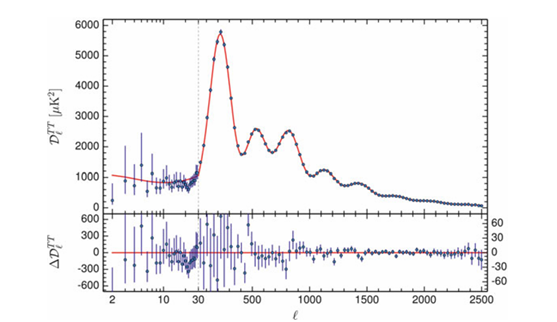
\includegraphics[scale=0.7]{Screenshot 2025-11-07 090025.png}
\end{center}

\section{Necessità di introdurre la materia oscura}

Riassiumiamo quello che abbiamo imparato, facendo il grafico del comportamento delle fluttuazioni con $a$, prendendo 3 fluttuzioni di massa via via crescente. Ci concentriamo in particolare su come appaiono al tempo della ricombinazione (CMB) e come appaiono oggi. 

\begin{enumerate}
    \item fluttuazioni di scala piccola \\
    Queste entrano nell'orizzonte prima dell'equivalenza, ed oscillano finchè non vengono completamente smorzate. Queste dunque non sono visibili nells radiazione di fondo e non hanno effetti oggi. 
    \item fluttuazioni grandi \\
    Entrano nell'orizzonte poco prima della riconbinazione: oscillano fino ad arrivare alla riconbinazione, dove poi ricontinuano a crescere. Naturalmente è fondamentale la fase con cui arrivano alla riconbinazione: se sono negative continueranno a crescere come lacune. 
    \item fluttuazioni ancora più grandi  \\
    Entrano nell'orizzonte dopo l'età dell'equivalenza: non oscillano e continuano a crescere. 
\end{enumerate}


La figura riassume la discussione:


\begin{center}
\begin{tikzpicture}[scale=0.7]
    \begin{axis}[
        xmin = 0, xmax = 2,
        ymin = -2, ymax = 2,
        xlabel = {$a(t)$},
        ylabel = {$\rho_i(a)$},
        grid = both,                % griglia
        grid style = {dashed, gray!30},
        axis lines = left,          % assi più puliti
        legend style={at={(0.98,0.98)},anchor=north east}, % legenda in alto a dx
        legend cell align={left},
        thick, % linee più spesse
    ]
        \addplot[color=red,   domain=0:0.25]{2*x} node[pos=0.35, above, sloped] {\small small $\lambda$};
        \addplot[color=red,   domain=0.25:1.5, samples=100]{0.5 + 1.5*sin(deg(4*pi*(x-0.25)))*exp(-2*x)};
        \addplot[color=red,   domain=1.5:2]{0.5}; 


        \addplot[color=blue,   domain=0:0.5]{x} node[pos=0.85, above, sloped] {\small large $\lambda$};
        \addplot[color=blue,   domain=0.5:1.5, samples=100]{0.5 + 0.8*sin(deg(4*pi*(x-0.5)))};
        \addplot[color=blue,   domain=1.5:2]{0.5 + (x-1.5)}; 

        \addplot[color=orange]{x/2}; 
        

        \begin{pgfonlayer}{background}
            \fill[blue!10]  (axis cs:0,-2)   rectangle (axis cs:0.5,2);
            \fill[green!10] (axis cs:0.5,-2) rectangle (axis cs:1.5,2);
            \fill[gray!10] (axis cs:1.5,-2) rectangle (axis cs:2,2);
        \end{pgfonlayer}


        
        % --- Note sul grafico ---
        \node at (axis cs:0.25, 1.7) {\small Era della};
        \node at (axis cs:0.25, 1.4) {\small radiazione};
        \node at (axis cs:1,1.8) {\small Era della materia};
        \node at (axis cs:1.75, 1.5) {\small Dopo la};
        \node at (axis cs:1.65, 1.2) {\small ricombinazione};
    \end{axis}
\end{tikzpicture}
\end{center}


Ora, nel 1990 si ebbero le prime misure della disomogeneità della radiazione cosmica di fondo. Si scoprì che vale $\delta \simeq 10^{-4}/10^{-5}$. Nel regime adiabatico, vale la \emph{relazione adiabatica}, che lega le fluttuazioni della radiazioni alle fluttuazioni della materia: 
\begin{equation}
    \frac{1}{4}\delta_{\gamma} = \frac{1}{3}\delta_m
\end{equation}

Facciamo un piccolo calcolo di quanto dovrebbe essere l'estremo superiore delle fluttuazioni, oggi. Sappiamo che al massimo, in universo di $\mathcal{E}dS$, vale 
\begin{equation}
    \frac{\delta_{oggi}}{\delta_{CMB}} \propto \frac{a_{oggi} = 1}{a_{ric}} \simeq 10^{3}
\end{equation}

Poichè sappiamo che vale circa $a_{ric} = 10^{-3}$. Questo è in pieno contrasto con le misure odierne, che invece ci dicono 

\begin{equation}
    \delta \simeq 1
\end{equation}

Di fatto, già c'era scetticismo verso questa teoria delle fluttuazioni anche prima di queste evidenze. Le scuole sovietiche e anglo-americane avevano cercato diversi espedienti per modificare queste teorie e renderle più plausibili. Questi prevedevano universi a "pankakes" che poi si sfilacciavano a creare le galassie. Questo però sembrava non creare in tempo le strutture che vediamo oggi. L'idea anglo-americana era invece di considerare un processo isotermo, e non adiabatico. Questo si sposa bene con il problema delle perturbazioni, perchè non valendo la relazione adiabatica, le fluttuazioni nella materia possono essere molto più grandi di quelle della materia relativistica. Queste teorie furono successivamente abbandonate. \\

Le fluttuazioni della CMB non sono l'unico problema di un universo composto solo da materia barionica e relativistica. Gia dagli anni '30, Zwicky osservò che la distribuzione delle velocità delle galasse nell'amasso della chioma di Berenice non era compatibile con la densità di materia deducibile dalla sua luminosità. Trovo che la materia doveva essere $7.8$ volte la massa dedotta. \\

Negli anni '70, Rubin osservò che le curve di rotazione delle galassie a spirale erano incompatibili con la massa osservata. Ancora una volta, la massa totale doveva essere circa $7$ volte la massa osservata. \\

Questo è in diretto scontro con le misure sulle abbondanze nella nucleosintesi primordiale: in pratica, le abbondanze di Deuterio, He$^3$,He$^4$, Li$^7$ dipendono tutte da un solo parametro, $\Omega_m$. Il solo modo per metterle d'accordo è dire 

\begin{equation}
    \Omega_{Bar} \leq 0.05
\end{equation}

che però a questo punto è in contrasto con le distribuzioni di velocità osservate. \\

L'ipotesi dunque è che vi sia una grande quantità di materia non barionica, che non emetta radiazione elettromagnetica, ma interagisca gravitazionalmente. Questa è detta materia \emph{oscura}. La domanda naturale è da quali particelle questa sia costituita. \\

Vi sono due modelli in particolare: 

\begin{enumerate}
    \item Materia oscura calda \\
    Si tratta di materia che rimane relativistica per molto tempo. Storicamente, questo modello è stato preso in considerazione per il sospetto che la materia oscura fosse costituita da neutrini. In particolare, dei calcoli suggerivano che se la massa del neutrino fosse stata $ \sim 30  \text{eV}$ allora questo giustificava la massa totale di materia oscura. Naturalmente oggi sapiamo che la massa dei neutrini, seppur finita, è molto minore. Inoltre, diventando non relativistici molto tardi, non fanno in tempo a creare le strutture che osserviamo oggi (proprietà detta \emph{free streeming}). 
    \item Materia oscura fredda \\
    è il modello adattato dal modello cosmologico standard attuale (che si chiama infatti $\Lambda$CDM), dove si suppone che valga $p \sim 0$, similmente alla materia barionica. Si suppone che questa interagisca anche con la forza nucleare debole, in quanto la massa scala di questa forza è precisamente in grado di giustificare la massa osservata di materia oscura (fatto noto come il miracolo WIMP, \emph{weakly interacting massive particles}). 
\end{enumerate}

Vorremmo capire allora come evolvono le perturbazioni della materia oscura (DM), ad esempio nell'era della radiazione. Ricordando che questa \emph{non interagisce} con la radiazione, non dobbiamo tenere conto della pressione (a differenza di quanto abbiamo fatto per la materia barionica). Questo in pratica permetterà alle fluttuazioni di non oscillare. Scriviamo dunque l'eq. di crescita: 

\begin{equation}
    \ddot{\delta}_{DM} + 2H\dot{\delta} = 4\pi G \rho_{DM}\delta_{DM}
\end{equation}

Introduciamo un paramentro che permette di scrivere l'eq. in un modo più comodo: sappiamo che $\rho_{tot} = \rho_\gamma + \rho_{DM} = \rho_{0\gamma}a^{-4} + \rho_{0m}a^{-3}$. All'equivalenza, i due contribuiti si equivalgono. In particolare varrà 
\begin{equation}
    \frac{\rho_{0m}}{\rho_{o\gamma}} = a_{eq}^{-1}
\end{equation}

Definisco allora 
\begin{equation}
    y = \frac{\rho_\gamma}{\rho_{DM}} = \frac{a}{a_{eq}}
\end{equation}

Indicando con $\delta' = \frac{d\delta}{dy}$, scriveremo l'eq. di crescita come 

\begin{equation}
    \delta''_{DM} + \frac{2+3y}{2y(1+y)}\delta'_{DM} - \frac{3}{2y(1+y)}\delta_{DM} = 0
\end{equation}

La cui soluzione ha un modo crescente dato da 

\begin{tcolorbox}[colback=gray!15, colframe=black, boxrule=1pt]
\begin{equation}
    \delta^+ = 1 + \frac{3}{2}y = 1+ \frac{3}{2}\frac{a}{a_{eq}}
\end{equation}
\end{tcolorbox}

Questo ci dice che il comportamento delle fluttuazioni di materia oscura ha due comportamenti diversi: 

\begin{enumerate}
    \item $a << a_{eq}$ \\
    Si ha che di fatto $\delta^+ \simeq cost. $. La perturbazione è dunque congelata fino all'equivalenza. 
    \item $a >> a_{eq}$ \\
    In questo regime, le fluttuazioni crescono con $\delta^+ \propto a$. 
\end{enumerate}

Ora, queste creano delle buche di potenziale. Qualitativamente, ci aspettiamo che la materia barionica caschi dentro queste buche, e si organizzi all'interno di questo scheletro fornito dalla materia oscura. Questo è un punto molto delicato, perchè quello che noi osserviamo è proprio la materia barionica. Vediamo dunque in dettaglio cosa succede, risolvendo l'eq. di crescita per le perturbazioni barioniche in questo regime: \\

L'equazione è data da 
\begin{equation}
    \ddot{\delta}_B  + 2H\dot{\delta} = 4\pi G \rho_{DM}\delta_{DM}
\end{equation}

Si osservi che l'eq. in presenza di materia oscura si modifica, in particolare cambia il termine di sorgente del potenziale gravitazionale. Avendo risolto l'eq. per la materia oscura, sappiamo che nell'era della materia vale $\delta_{DM} = Ba$ e possiamo risolvere anche questa, passando però $\delta(t) \rightarrow \delta(a)$. \\

Per fare il cambio di coordinate, bisogna comprendere come cambiano le derivate: 

\begin{equation}
    \frac{d}{dt} = \dot{a}\frac{d}{da}
\end{equation}

Questo vuol dire che 
\begin{equation}
    \dot{\delta} = \dot{a}\delta'
\end{equation}
e in particolare poi 
\begin{equation}
    \ddot{\delta} = \dot{a}^2 \delta'' + \delta' \dot{a}\frac{d}{da}\dot{a}
\end{equation}

Scrivendo 
\begin{equation}
    \frac{d}{da} = \frac{1}{\dot{a}}\frac{d}{dt}
\end{equation}
otteniamo allora che 
\begin{equation}
    \ddot{\delta} = \dot{a}^2 \delta'' + \delta' \ddot{a}
\end{equation}

Ora, uno può esprimere anche $\dot{a}, \ddot{a}$ in funzione di $a$, una volta che è nota la relazione $t = t(a)$. Se siamo nell'era della materia, in particolare, sappiamo che 
\begin{equation}
    a(t) = \left(\frac{3}{2}H_0 \right)^{2/3}t^{2/3}
\end{equation}

Derivando e sostituendo troviamo che 
\begin{align}
    &\dot{a} = H_0a^{-1/2} \\ &\ddot{a} = -\frac{1}{2}H_0^2 a^{-2}
\end{align}

L'unico pezzo che ci manca ce lo fornisce la prima eq. di Friedmann: $4\pi G \rho = \frac{3}{2}H_0^2 a^{-3}$, così che infine scriveremo 

\begin{equation}
    a\delta'' + \frac{3}{2}\delta' = \frac{3}{2}B
\end{equation}

Una soluzione dell'equazione è data da 
\begin{equation}
    \delta_B = B(a - c)
\end{equation}

Dove $c$ è una costante di integrazione, da determinarsi a partire dalle condizioni iniziali. Ma siccome stiamo risolvendo l'eq. nell'età della materia, la condizione iniziale è la densità di materia barionica alla riconbinazione. In prima approssimazione, considerando gli effetti del silke-damping, possiamo quindi prendere $\delta_B(a_{ric}) \simeq 0$. In questo caso otteniammo 

\begin{tcolorbox}[colback=gray!15, colframe=black, boxrule=1pt]
\begin{equation}
    \delta_B = B(a - a_{ric}) = Ba\left(1 - \frac{a_{ric}}{a}\right) = \delta_{DM}\left(1 - \frac{a_{ric}}{a}\right)
\end{equation}
\end{tcolorbox}

Come prima osservazione, vediamo che 
\begin{equation}
    \delta_{B}(a=1) = \delta_{DM}(1 - 10^3) \simeq \delta_{DM}
\end{equation}

In effetti, già per $a=10^{2}$, si ottiene che $\delta_B \simeq 0.9\delta_{DM}$. Cioè le perturbazioni della materia barionica tendono ad uniformarsi abbastanza velocemente alle perturbazioni della materia oscura, anche se le prime si erano annullate alla ricombinazione! Questo permette ad esempio di dire che lo spettro di potenza delle galassie coincide con quello della materia oscura, a meno chiaramente di un fattore di bias (che effettivamente può diventare rognoso a scale piccole, dove interviene anche un bias quadratico). \\

Cosa succede invece se $\delta_B(a_{ric}) \neq 0$? In effetti, essendo il comportamento oscillante, potremmo avere sia $\delta_B(a_{ric}) >0$, sia $\delta_B(a_{ric}) <0$. Di fatto, questa puòp essere una piccola frazione della materia oscura, che comunque ne risente gravitazionalmente. Questo crea delle piccole oscillazioni nello spettro di potenza. \\

Torniamo a parlare proprio dello spettro di potenza: alla luce delle nostre osservazioni, siamo in grado di spiegare in modo qualitativo ma anche molto soddisfaciente la forma dello spettro di potenza che osserviamo sperimentalmente. \\

A scale basse, l'inflazione prevede che lo spettro di potenza segua una legge del tipo $P_0(k) \propto k$. Le misure ci dicono che se fittiamo lo spettro di potenza con una legge di potenza, $p = k^n$, allora si trova $n = 0.96 \pm 0.01$.  

\begin{multicols}{2}

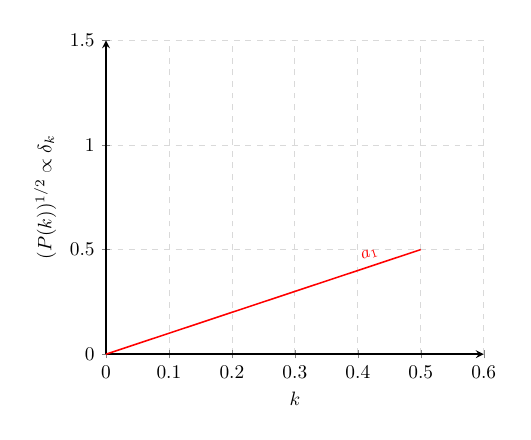
\begin{tikzpicture}[scale=0.7]
    \begin{axis}[
        xmin = 0, xmax = 0.6,
        ymin = 0, ymax = 1.5,
        xlabel = {$k$},
        ylabel = {$(P(k))^{1/2}\propto \delta_k$},
        grid = both,                % griglia
        grid style = {dashed, gray!30},
        axis lines = left,          % assi più puliti
        legend style={at={(0.98,0.98)},anchor=north east}, % legenda in alto a dx
        legend cell align={left},
        thick, % linee più spesse
    ]
        \addplot[color=red,   domain=0:0.5, samples=2]{x} node[pos=0.85, above, sloped] {\small $a_1$};
        
    \end{axis}
\end{tikzpicture}

\columnbreak
Facciamo un grafico di $(P(k))^{1/2} \propto \delta_k$, ad un tempo $a_1$: otterremo la figura rappresentata a destra. \\
Questo perchè arrivato ad una certa lunghezza d'onda, che chiamo $k_h$, la perturbazione entra nell'orizzonte, e si congela. 
\end{multicols}

\begin{multicols}{2}

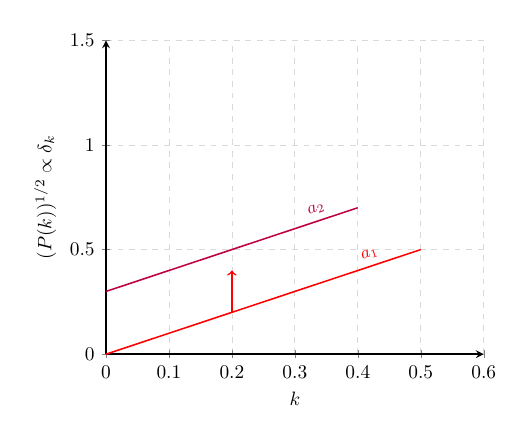
\begin{tikzpicture}[scale=0.7]
    \begin{axis}[
        xmin = 0, xmax = 0.6,
        ymin = 0, ymax = 1.5,
        xlabel = {$k$},
        ylabel = {$(P(k))^{1/2}\propto \delta_k$},
        grid = both,                % griglia
        grid style = {dashed, gray!30},
        axis lines = left,          % assi più puliti
        legend style={at={(0.98,0.98)},anchor=north east}, % legenda in alto a dx
        legend cell align={left},
        thick, % linee più spesse
    ]
        \addplot[color=red,   domain=0:0.5, samples=2]{x} node[pos=0.85, above, sloped] {\small $a_1$};
        \draw[->, thick, red] (axis cs:(0.2,0.2) -- (axis cs:0.2,0.4);

        \addplot[color=purple,   domain=0:0.4, samples=2]{x+0.3} node[pos=0.85, above, sloped] {\small $a_2$};
        
    \end{axis}
\end{tikzpicture}

\columnbreak
Ora consideriamo il tempo $a_2 > a_1$. L'orizzonte si sposta col tempo, perchè vale $r_H \propto t \propto a^2 \rightarrow r_H^{com} \propto a \rightarrow k_H \propto \frac{1}{a}$. La perturbazione allora entra prima nell'orizzonte, e si congela prima. D'altra parte questa è più grande della precedente per effetto della crescita, di un fattore $(a_2/a_1)^2$.  

\end{multicols}

\begin{multicols}{2}

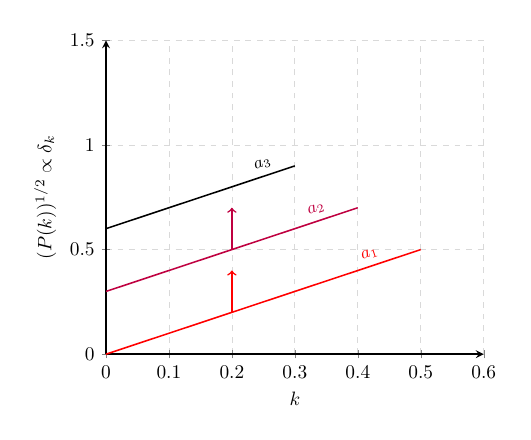
\begin{tikzpicture}[scale=0.7]
    \begin{axis}[
        xmin = 0, xmax = 0.6,
        ymin = 0, ymax = 1.5,
        xlabel = {$k$},
        ylabel = {$(P(k))^{1/2}\propto \delta_k$},
        grid = both,                % griglia
        grid style = {dashed, gray!30},
        axis lines = left,          % assi più puliti
        legend style={at={(0.98,0.98)},anchor=north east}, % legenda in alto a dx
        legend cell align={left},
        thick, % linee più spesse
    ]
        \addplot[color=red,   domain=0:0.5, samples=2]{x} node[pos=0.85, above, sloped] {\small $a_1$};
        \draw[->, thick, red] (axis cs:(0.2,0.2) -- (axis cs:0.2,0.4);

        \addplot[color=purple,   domain=0:0.4, samples=2]{x+0.3} node[pos=0.85, above, sloped] {\small $a_2$};
         \draw[->, thick, purple] (axis cs:(0.2,0.5) -- (axis cs:0.2,0.7);

        \addplot[color=black,   domain=0:0.3, samples=2]{x+0.6} node[pos=0.85, above, sloped] {\small $a_3$};
        
    \end{axis}
\end{tikzpicture}

\columnbreak
Ora consideriamo un tempo corrispondente da $a_3=a_{eq}$. Questo è di fatto l'ultima era in cui vi è congelamento: da qui in avanti, vi è uno spostamento rigido verso l'alto delle fluttuazioni. 
\end{multicols}

\begin{multicols}{2}

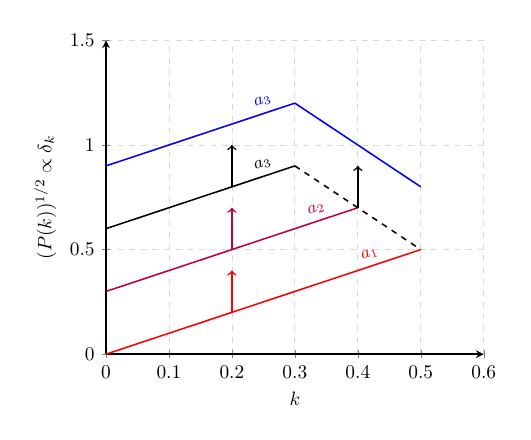
\begin{tikzpicture}[scale=0.7]
    \begin{axis}[
        xmin = 0, xmax = 0.6,
        ymin = 0, ymax = 1.5,
        xlabel = {$k$},
        ylabel = {$(P(k))^{1/2}\propto \delta_k$},
        grid = both,                % griglia
        grid style = {dashed, gray!30},
        axis lines = left,          % assi più puliti
        legend style={at={(0.98,0.98)},anchor=north east}, % legenda in alto a dx
        legend cell align={left},
        thick, % linee più spesse
    ]
        \addplot[color=red,   domain=0:0.5]{x} node[pos=0.85, above, sloped] {\small $a_1$};

        \draw[->, thick, red] (axis cs:(0.2,0.2) -- (axis cs:0.2,0.4);

        \addplot[color=purple,   domain=0:0.4]{x+0.3} node[pos=0.85, above, sloped] {\small $a_2$};

        \draw[->, thick, purple] (axis cs:(0.2,0.5) -- (axis cs:0.2,0.7);

        \addplot[color=black,   domain=0:0.3]{x+0.6} node[pos=0.85, above, sloped] {\small $a_3$};

        \draw[->, thick, black] (axis cs:(0.2,0.8) -- (axis cs:0.2,1.0);

        \draw[->, thick, black] (axis cs:(0.4,0.7) -- (axis cs:0.4,0.9);

        \addplot[color=black, dashed, domain = 0.3:0.5]{-2*x + 1.5}; 

        \addplot[color=blue,   domain=0:0.3]{x+0.9} node[pos=0.85, above, sloped] {\small $a_3$};
        \addplot[color=blue,   domain=0.3:0.5]{-2*x+1.8}; 
        
    \end{axis}
\end{tikzpicture}

\columnbreak
Infine, consideriamo $a_4 > a_{eq}$. Dopo l'equivalenza, tutte le perturbazioni si "disgelano", così che la forma dello spettro sarà un triangolo (nella realtà un po' smussato). 
\end{multicols}

Per completezza alleghiamo un fit dei dati sperimentali dello spettro di potenza (sempre in scala logaritmica): 
\begin{center}
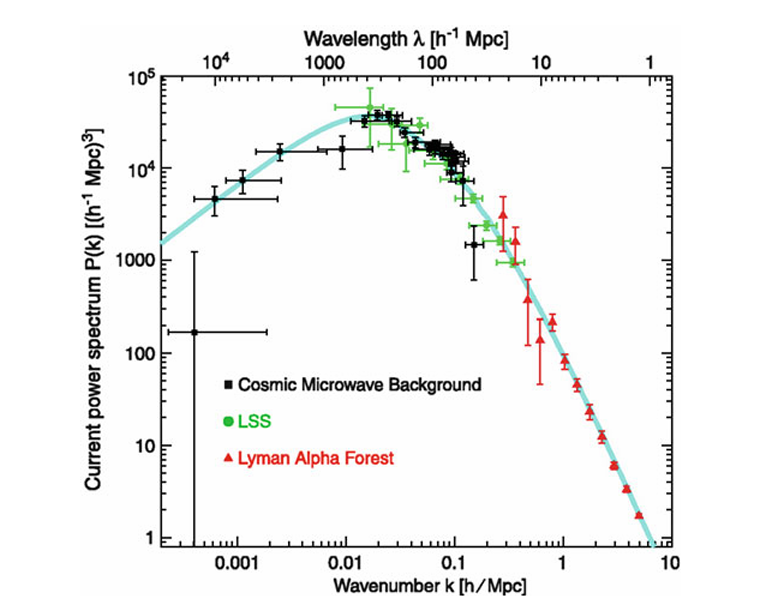
\includegraphics[scale = 0.4]{Screenshot 2025-11-07 085511.png}
\end{center}

Due commenti sul grafico: 

\begin{enumerate}
\item Si noti la posizione del picco, situato a $k_{eq}$, cioè il numero d'onda della fluttuazione che entra nell'orizzonte precisamente nell'età dell'equivalenza. Essendo legato ad $a_{eq}$ dipende fortemente da $\rho_{0\gamma}, \rho_{0m}$ e dunque la sua posizione implica diversi vincoli sui parametri cosmologici. 
\item Data la pendenza della prima parte dello spettro, possiamo dire qualcosa sulla seconda parte? In effetti si: senza il congelamento della perturbazione, anche per $k>k_{eq}$ avremmo avuto $\delta_k \propto k^{n/2}$. Siccome mi sono congelato, devo correggere moltiplicando per il rapporto (al quadrato, perchè così crescono le perturbazioni nell'età della materia) fra i fattori di scala: $(a/a_{eq})^2$. Scriveremo allora 

\[\begin{cases}
    \delta_k \propto k^{n/2} \quad k< k_{eq}\\
    \delta_k \propto k^{n/2}\left[\frac{a}{a_{eq}}\right]^2 \quad k> k_{eq} 
\end{cases}\]

D'altra parte, abbiamo già osservato che $a \propto \frac{1}{k}$. Questo infine impilca 

\[\begin{cases}
    \delta_k \propto k^{n/2} \rightarrow P(k) \propto k^n\quad k< k_{eq}\\ 
    \delta_k \propto k^{n/2}k^{-2} \rightarrow P(k) \propto k^{n-4}\quad k> k_{eq} 
\end{cases}\]

In particolare, se $n \simeq 1$, allora nella seconda parte dello spettro varrà $P(k) \propto k^{-3}$. Questo è in pieno accordo con i dati sperimentali. 
\end{enumerate}

\section{Spettro di potenza della CMB}

Come già descritto, le perturbazioni della radiazione cosmica di fondo sono espressi in polinomi di Legendre. Riportiamo nuovamente lo spettro di potenza ricavato da PLANK, nel 2015: 

\begin{center}
    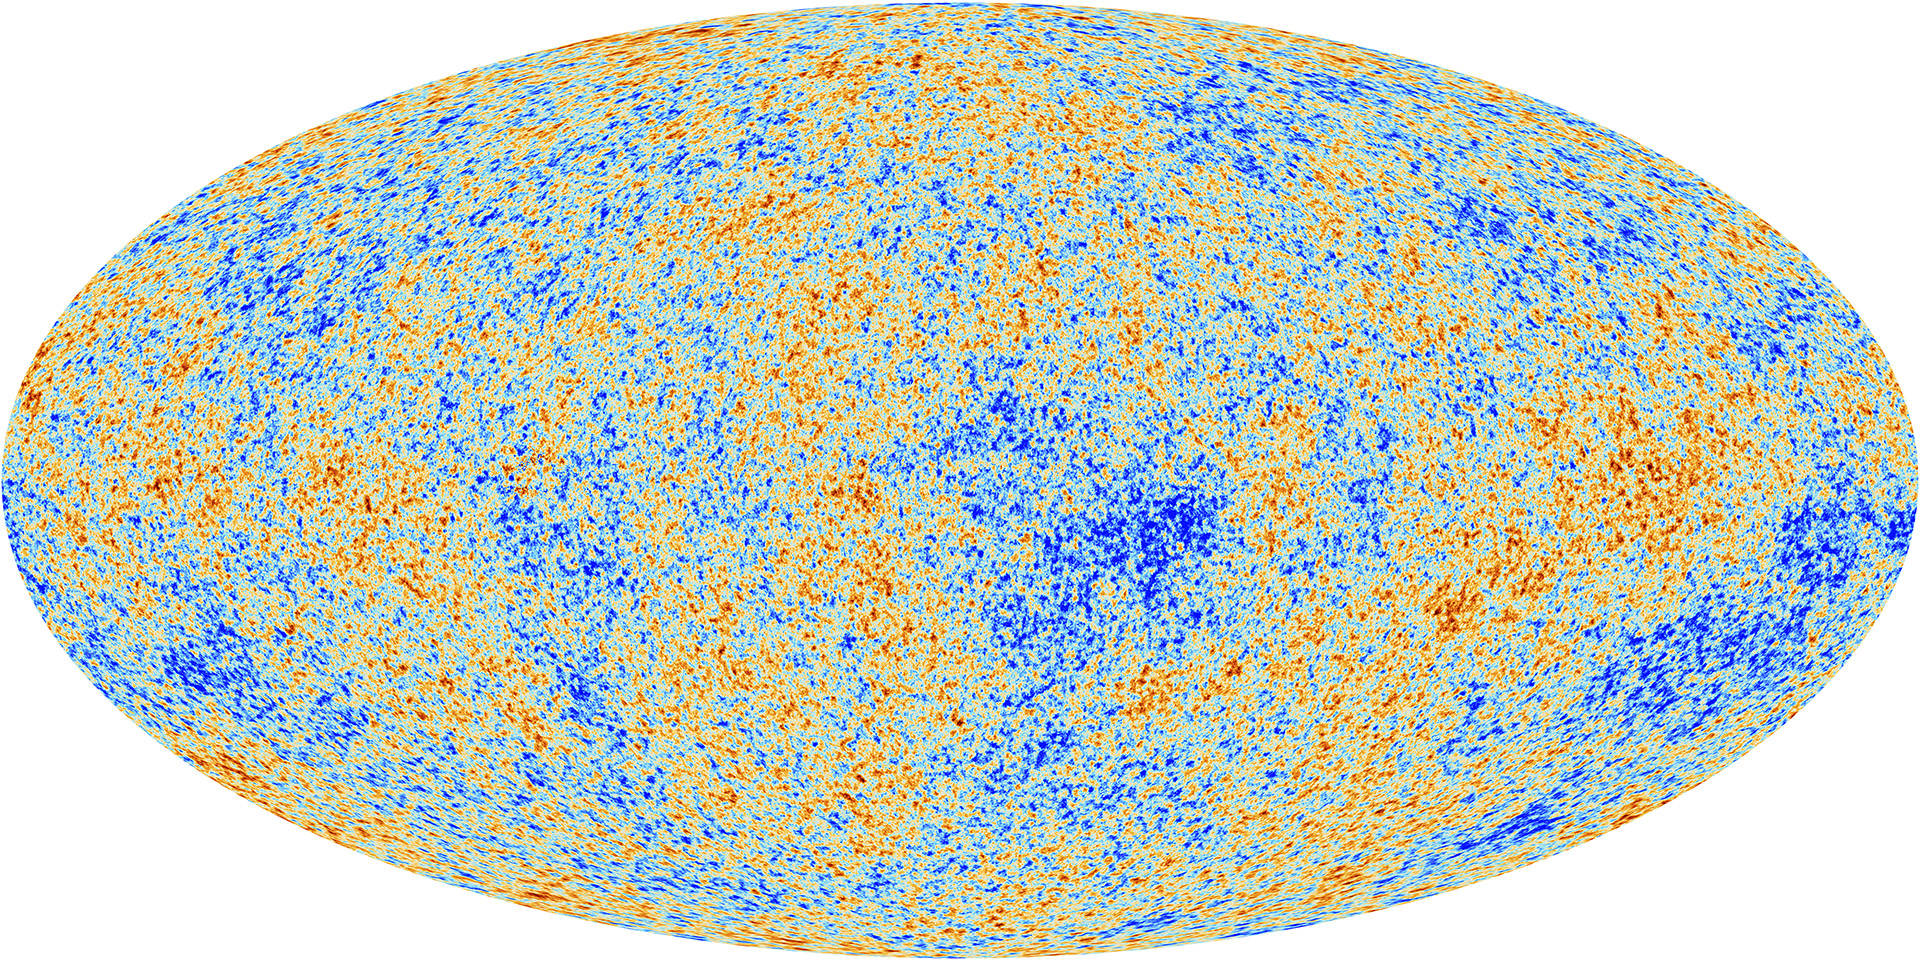
\includegraphics[scale=0.15]{Planck_CMB.jpg}
\end{center}

\begin{center}
    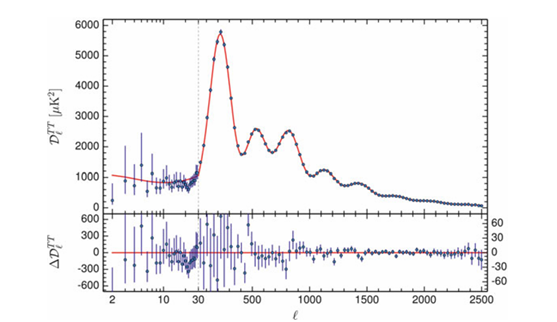
\includegraphics[scale=0.8]{Screenshot 2025-11-07 090025.png}
\end{center}

Da cosa sono date le oscillazioni che misuriamo? Di fatto, sono date dalla somma di 3 contributi: 
\begin{enumerate}
    \item Le fluttuazioni in densità di materia
    \item Effetto doppler 
    \item Red-shift gravitazionale
\end{enumerate}

Occupiamoci dunque in dettaglio di come contribusicono le fluttuazioni in densità sullo spettro della CMB: \\
Torniamo a considerare il comportamento dei barioni prima della riconbinazione: sappiamo che per effetto della pressione fornitagli dai fotoni questi oscillano. D'altra parte, con la presenza della materia oscura, questi risentono del potenziale gravitazionale creato dalle perturbazioni di questa. Risolviamo allora nel dettaglio l'equazione per la materia barionica in questo regime, considerando il contributo della materia oscura: \\

Dobbiamo risolvere l'eq. lineare di crescita: 

\begin{equation}
    \ddot{\delta}_k + 2H\dot{\delta} + (c_s^2k^2 - 4\pi G\rho)\delta_k = 0 
\end{equation}

Per il momento, dimentichiamoci del termine di smorzamento, tanto sappiamo la funzione che ha nell'espressione. Potremmo rendere questo più rigoroso dicendo che consideriamo perturbazioni che hanno un periodo molto più piccolo dell'inverso della costante di Hubble. Prendiamo anche $\lambda << \lambda_j$\\

In queste condizioni, l'eq. (nello spazio di Fourier) assume la forma 

\begin{equation}
    \ddot{\delta}_k + k^2c_s^2\delta_k = F_k
\end{equation}

Dove $F_k$ è il contributo della materia oscura, dato da 
\begin{equation}
    F_k = \mathcal{F}(4\pi G \rho \delta_{DM})
\end{equation}

Ricordandomi dell'eq. di Possion, scrivo 
\begin{equation}
    4\pi G \rho \delta_{DM} = \frac{1}{a^2}\nabla^2 \phi'
\end{equation}

In letteratura la perturbazione del potenziale newtoniano si scrive spesso anche $\psi$, e cominciamo a chiamarla anche noi così. Tornando al nostro problema, 

\begin{equation}
    F_k = \mathcal{F}\left(\frac{1}{a^2}\nabla^2 \psi\right) = -\frac{k^2}{a^2}\psi_k = -k_p^2 \psi_k
\end{equation}

Ora ci ricordiamo che all'interno dell'eq. di crescita abbiamo sempre indicato con $k$ il numero d'onda \emph{fisico}, e smettiamo di scrivere il pedice. L'eq. da risolvere è dunque 

\begin{equation}
    \ddot{\delta}_k + k^2c_s^2 \delta_k = -k^2\psi_k
\end{equation}

Che come soluzione ha un oscillazione shiftata verso il basso: 

\begin{equation}
    \delta_k(t) = \left(\delta_{H_k}  + \frac{\psi_k}{c_s^2}\right)\cos{(c_skt)} - \frac{\psi_k}{c_s^2}
\end{equation}

Definiamo ora l'\emph{orizzonte sonoro alla riconbinazione}, dato da 
\[\begin{cases}
    s_p = c_st_{ric} \quad (\text{fisico}) \\ s = c_s\tau_{ric} \quad (\text{comovente})
\end{cases}\]

Questo dà di fatto la massima ampiezza di una perturbazione all'epoca della ricombinazione. 

Scrivendo la nostra soluzione, al tempo della riconbinazione, introducendo $s$, possiamo vederla come una funzione del numero d'onda dell'oscillazione $k$: 

\begin{equation}
    \delta_k(\tau)|_{\tau = \tau_{ric}} = \left(\delta_{H_k}  + \frac{\psi_k}{c_s^2}\right)\cos{(sk)} - \frac{\psi_k}{c_s^2}
\end{equation}

Ora mi ricordo che lo spettro di potenza $P(k)$ è proporzionale al quadrato della perturbazione, e mi rendo conto che varrà 

\begin{equation}
    P(k) \propto \cos^2(sk) -2\left(\frac{\psi_k}{c_s}\right)\cos(sk) + \left(\frac{\psi_k}{c_s} \right)^2
\end{equation}

Questo marca un effetto che è perfettamente visibile nello spettro di potenza: poichè il coseno al quadrato ha il periodo che è la metà del coseno, in alternanza, i picchi dei due sono concordi o discordi. Questo fa si che nello spettro sia visibile un pattern di picco alto, picco basso, picco alto, picco basso, ecc. Naturalmente questo è più visibile nella prima parte dello spettro quando si sente meno l'effetto del Silke-damping. \\

Queste perturbazioni sono legate alle perturbazioni in temperatura mediante la formula 
\begin{align}
    \left(\frac{\delta T}{T}\right)^{\text{Potenziale}} &= \frac{1}{3}\delta \\
     \left(\frac{\delta T}{T} \right)^{\text{Potenziale}}_k&= \frac{1}{3}\left(\delta_{H_k}  + \frac{\psi_k}{c_s^2}\right)\cos{(c_sk\tau)} - \frac{1}{3}\frac{\psi_k}{c_s^2}
\end{align}

Per dare informazioni più quantitative, dobbiamo tenere conto anche del contributo dell'effetto doppler e del red shift gravitazionale. Questi hanno un contributo non nullo dato da:

\begin{enumerate}
    \item Red shift gravitazionale \\
    I fotoni non sono emessi da uno spazio piatto, ma capita che debbano risalire le buche di potenziale create dalle perturbazioni. Questo fa sì che questi perdano energia, e vi sia red-shift. 
    \item Effetto doppler \\
    La materia che emette i fotoni non è statica, ma ha una sua certa velocità quando la perturbazione si espande o si contrae. Nel primo caso, il fotone emesso subirà blue-shift, nel secondo red-shift. 
\end{enumerate}

Questi effetti sono noti come \emph{asintropie primarie}. In linea di principio,  dovremmo anche tenere conto delle cosiddette \emph{asintropie secondarie}, che sono dovute a tutti gli ostacoli che i fotoni incontrano prima di giungere a noi (e.g. galassie, gas caldi, ecc.). Per semplicità non considereremo questi effetti, che incidono in modo meno significativo dei primi.\\

Il red-shift gravitazionale è un argomento molto avanzato, che richiede conti in gravità generale, e non lo tratteremo. Il termine di effetto Doppler, invece, è semplice da capire, una volta che siamo in grado di determinare il campo di velocità associato ad un campo di fluttuazione. \\


Ora per determinare il campo di velocità a partire dalle fluttuazioni è sufficiente usare l'eq. di continuità (linearizzata): 

\begin{equation}
    \vec{\nabla}\cdot \vec{v} = -a\frac{\partial \delta}{\partial t}
\end{equation}

Scriviamo questa nello spazio di Fourier: un teorema assicura che  
\begin{equation}
    \mathcal{F}(\vec{\nabla}\cdot \vec{v}) = i\vec{k}\cdot \mathcal{F}(\vec{v})
\end{equation}
Dove con $\mathcal{F}(\vec{v})$ indichiamo il vettore che ha per componenti la trasformata di fourier delle componenti del vettore $\vec{v}$. Per comodità da ora in poi lo denoteremo $\vec{v}_k$,  in formule
\begin{equation}
    \mathcal{F}(\vec{v}) = (\mathcal{F}(v_x), \mathcal{F}(v_y), \mathcal{F}(v_z)) = \vec{v}_k
\end{equation}

Ora dalla geometria della trasformata di Fourier è chiaro che i vettori $\vec{k}, \vec{v}$ sono paralleli, così che scriveremo 
\begin{equation}
    ikv_k = -\frac{1}{a}\frac{\partial \delta_k}{\partial t} = -\frac{\partial \delta_k}{\partial \tau}
\end{equation}

Calcolo

\begin{equation}
    \frac{\partial \delta_k}{\partial \tau} = -c_sk\left(\delta_{H_k} + \frac{\psi_k}{c_s^2}\right)\sin(c_sk\tau)
\end{equation}

da cui deduco: 

\begin{equation}
    v_k = ic_s\left(\delta_{H_k} + \frac{\psi_k}{c_s^2}\right)\sin(c_sk\tau)
\end{equation}

Che vuol dire che la velocità come vettore si scrive 
\begin{equation}
    \vec{v_k} = ic_s\left(\delta_{H_k} + \frac{\psi_k}{c_s^2}\right)\sin(c_sk\tau)\hat{k}
\end{equation}

L'effetto doppler sarà prorzionale al prodotto fra la velocità ed il versore che indica la direzione dove noi osserviamo la radiazione emessa: senza dimostrazione, enunciamo che vale 

\begin{equation}
    \left(\frac{\delta T}{T}\right)^{\text{Doppler}} = \frac{|v|}{c}\cos \theta
\end{equation}

Che unito alla nostra formula per la velocità ci dice infine 
\begin{equation}
    \left(\frac{\delta T}{T} \right)^{\text{Doppler}}_k = i\frac{c_s}{c}\left(\delta_{H_k} + \frac{\psi_k}{c_s^2}\right)\sin(c_sk\tau)\cos\theta
\end{equation}

Enunciamo invece il risultato per il red shift gravitazionale: 
\begin{equation}
    \left(\frac{\delta T}{T} \right)_k^{\text{red-shift}} \simeq \frac{1}{3}\frac{\psi_k}{c_s^2}
\end{equation}

Troviamo dunque infine, facendo la somma dei tre contributi, che 
\begin{tcolorbox}[colback=gray!15, colframe=black, boxrule=1pt]
\begin{align}
    \left(\frac{\delta T}{T} \right)_k = \Theta_k = \frac{1}{3}\left(\delta_{H_k}  + \frac{\psi_k}{c_s^2}\right)\cos{(c_sk\tau)} + ic_s\left(\delta_{H_k} + \frac{\psi_k}{c_s^2}\right)\sin(c_sk\tau)\cos\theta
\end{align}
\end{tcolorbox}

Chiaramente, lo spettro di potenza sarà proporzionale al modulo quadro di questo termine. 

\section{Teoria lineare delle RDS}

Torniamo ora a considerare l'eq. di continuità linearizzata, che ricordiamo essere data da 
\begin{equation}
    \vec{\nabla}\cdot \vec{v} = -a\frac{\partial \delta}{\partial t}
\end{equation}

Ricordandomi che posso scrivere 
\begin{equation}
    \frac{\partial}{\partial t} = \dot{a}\frac{d}{da}
\end{equation}

e ricordandomi la definizione di $D = \delta^+/\delta_0$, scriveremo
\begin{equation}
    \vec{\nabla}\cdot \vec{v} = -a\dot{a}\delta_0\frac{\partial D}{\partial t}
\end{equation}

Moltiplico e divido per $D$: 
\begin{equation}
    \vec{\nabla}\cdot \vec{v} = -\dot{a}D\delta_0\frac{a}{D}\frac{\partial D}{\partial t} = -\dot{a}\delta f
\end{equation}

Dove abbiamo introdotto il parametro $f$, noto come \emph{tasso di crescita}, dato da 
\begin{equation}
    f = \frac{d \ln D}{d\ln a}
\end{equation}

Ora, noi tipicamente misuriamo $\delta_{gal}$, dalle red-shift surveys. Sappiamo che questa misura da' le fluttuazioni di materia meno un fattore di bias, che supponiamo essere lineare: 
\begin{equation}
    \delta_{gal} = b\delta
\end{equation}

Potremmo scrivere in termini di questa l'eq. di continuità, data da 
\begin{equation}
    \vec{\nabla}\cdot \vec{v}_{gal} = -\frac{aHf}{b}\delta_{gal}
\end{equation}

Vediamo dunque che se sappiamo $v_{gal}, \delta_{gal}$, allora otteniamo informazioni sul parametro 
\begin{equation}
    \beta = \frac{f}{b}
\end{equation}

Perchè questo è interessante? di fatto, possiamo scrivere l'eq. di crescita lineare in termini di $f$: 
\begin{equation}
    a\frac{df}{da} + f^2 \left(\frac{\dot{H}}{H^2} +2\right) = \frac{3}{2}\Omega_m
\end{equation}

Non sono note soluzioni analitiche di questa. Una soluzione approssimata è data da 
\begin{equation}
    f = \Omega_m^\gamma, \gamma \simeq 0.55
\end{equation}

Dunque, determinare $\beta$ è interessante perchè è di fatto proporzionale ad $\Omega_m$. \\

Ci sono però diversi problemi tecnici. Come posso misurare le velocità peculiari? Noi misuriamo un red-shift, che è dato dalla velocità con cui si sta allontanando una certa galassia. Questo è dato dalla somma del flusso di Hubble e dalla componente parallela della velocità peculiare. A meno che non ho un'altra misura della distanza, da cui posso dedurre l'effetto di red-shift cosmologico, non posso saparare i due contributi. Di fatto, l'unico modo in cui posso farlo è in presenza di candele standard (e.g. supernove di tipo 1A), e questo è il motivo per cui non ci sono misure di velocità peculiari per $cz < 20000 \, \text{km s}^{-1}$. \\

In effetti, questo è un problema. Quando io faccio una misura, per \(z <<1\), vale la legge di Hubble
\begin{equation}
    cz_{mis} = H_0r + \vec{v}\cdot \hat{r} = H_0 r_s
\end{equation}

Dunque la distanza che misuro differisce dalla distanza reale, attraverso 
\begin{equation}
    r = r_s - \frac{\vec{v}\cdot \hat{r}}{H_0}
\end{equation}
Questo effetto è noto come \emph{red shift distortions}. \\
Abbiamo visto la differenza fra \(r, r_s\) per red-shift piccoli. Per una teoria completa a distanze cosmologiche, doveremo calcolare la differenza fra le distanze comoventi. Questo è stato il punto di partenza di Kaiser,  che nell'87 sviluppò una teoria lineare nelle velocità peculiari, con lo scopo di legare lo spettro di potenza osservato da noi nello spazio di red-shift, con lo spazio reale. \\

La distanza comovente \emph{reale} tra noi e un oggetto a red-shift $z$ è data da: 
\begin{equation}
    r = \int_0^z \frac{cdz}{H(z)}
\end{equation}

mentre la distanza nello spazio di red-shift vale: \footnote{Nota che siccome adesso trattiamo di distanze comoventi, la velocità deve essere moltiplicata per \(1+z\), ovvero divisa per \(a\)}. 
\begin{equation}
    r_s = \int_0^{z + \frac{v_\parallel(1+z)}{c}}\frac{cdz}{H(z)} = r + \int_z^{z+\frac{v_\parallel(1+z)}{c}} \frac{cdz}{H(z)}
\end{equation}
Ora nell'ultimo integrale supponiamo che $H(z)$ non varii nell'intervallo di integrazione, così che avremo 
\begin{equation}
    r_s = r + \frac{v_{\parallel}}{aH(a)} = r + \frac{\vec{v} \cdot\hat{r}}{aH(a)} 
\end{equation}

Per comodità, scriviamo 
\begin{equation}
    \mu_{\parallel} = \frac{\vec{v} \cdot\hat{r}}{aH(a)}
\end{equation}

Ora, prendiamo un volumetto nello spazio reale e nello spazio di red-shift. Questi avranno una loro densità numerica di galassie $n(r), n_s(r_s)$ e volume $d^3r, d^3r_s$. Ora l'idea fondamentale è che le velocità peculiari spostano la posizione delle galassie, ma comunque il numero totale si conserva: possiamo allora scrivere 
\begin{equation}
    n(r)d^3r = n_s(r_s)d^3r_s 
\end{equation}
Se immagino i volumetti dei cilindretti, con la base data da $r^2d\Omega$, scriveremo che il loro volume è dato da 
\begin{equation}
    d^3r = dr r^2d\Omega
\end{equation}
Così che la condizione diventi 
\begin{equation}
    n(r)r^2dr = n_s(r_s)r_s^2 dr_s \rightarrow n(r) = n_s(r_s)\left(\frac{r_s}{r}\right)^2\frac{dr_s}{dr}
\end{equation}

Dalla relazione $r_s = r + \mu_{\parallel}$, troviamo che 
\begin{align}
    &\frac{dr_s}{dr} = 1 + \frac{\partial \mu_{\parallel}}{\partial t} \\
    &\left(\frac{r_s}{r}\right)^2 = \left(1+\frac{\mu_{\parallel}}{r} \right)^2
\end{align}
Passando dalle densità alle fluttuazioni di densità, è possibile ottenere un legame fra le fluttuazioni in spazio reale e di red-shift (che è proprio il nostro obbiettivo, perchè lo spettro di potenza è proporzionale alle fluttuazioni al quadrato). Nel dettaglio, possiamo scrivere 
\begin{align}
    &n(r) = \bar{n}(1+\delta(r)) \\ &n_s(r_s) = \bar{n}(1+\delta(r_s))
\end{align}

dove abbiamo sfruttato il fatto che il campione è lo stesso, e dunque avrà la stessa densità media. La nostra espressione diventa allora

\begin{equation}
    1 + \delta_s(r_s) = (1+\delta(r))\left(1+\frac{\mu_{\parallel}}{r} \right)^{-2}\left(1 + \frac{\partial \mu_{\parallel}}{\partial t} \right)^{-1}
\end{equation}

A questo punto viene comodo fare un approssimazione lineare, fermandoci ai temini lineari in $\mu_{\parallel}, \delta$, così da ottenere
\begin{equation}
    \delta_s(r) = \delta(r) - \frac{\partial u_{\parallel}}{\partial t}
\end{equation}

Lo sviluppo del lato destro è del tutto ovvio, mentre osserviamo che al lato sinistro avrei 
\begin{equation}
    1 + \delta_s(r_s) = 1 + \delta_s(r + \mu_{\parallel}) \simeq 1 + \delta_s(r) + \mu_{\parallel} \frac{\partial \delta}{\partial r } \simeq \ 1 + \delta_s(r)
\end{equation}

Ora, per ottenere informazioni sullo spettro di potenza devo passare nello spazio di Fourier: 

\begin{align}
    \delta_s(k) &= \int d^3r \delta_s(r)e^{-i\vec{k}\cdot \vec{r}} \\
    &= \int d^3r \left[\delta(r) - \frac{\partial \mu_{\parallel}}{\partial t}\right]e^{-i\vec{k}\cdot \vec{r}} \\
    &= \delta_k - \int d^3k \frac{\partial \mu_{\parallel}}{\partial t}e^{-i\vec{k}\cdot \vec{r}}
\end{align}

Rivolgiamo allora la nostra attenzione verso il fattore 
\begin{align}
    I_k = \int d^3k \frac{\partial \mu_{\parallel}}{\partial t}e^{-i\vec{k}\cdot \vec{r}}
\end{align}

Poichè $\mu_{\parallel}$ deriva dalla velocità, comincio col scrivere questa in anti-trasformata di Fourier: 
\begin{equation}
    \vec{v}(\vec{r}) = \frac{1}{(2\pi)^3}\int d^3k' \vec{v}(k')e^{i\vec{k'}\cdot \vec{r}}
\end{equation}

Ora mi ricordo che la componente k-esima della velocità posso ottenerla a partire della equazione di continuità, che avevamo scritto in termine del tasso di crescita $f$: 
\begin{equation}
    \vec{v}(k') = iHaf \frac{\delta(k')}{|k'|}\hat{k'}
\end{equation}

Sostituendo per $\mu_{\parallel}$, trovo 
\begin{equation}
    \mu_\parallel = \frac{iHaf}{aH(2\pi)^3}\int d^3k' \frac{\delta(k')}{|k'|^2}(\vec{k'}\cdot \hat{r})e^{i\vec{k'}\cdot \vec{r}}
\end{equation}

D'altra parte, noi siamo interessati a $\partial_r \mu_{\parallel}$. Come faccio a calcolarla? Devo fare un ipotesi, l'ipotesi di \emph{campo lontano}. In pratica, assumo che il volume che sto osservando copra un angolo talmente piccolo, che tutte le linee di vista posso considerarle parallele (in pratica, verticali). Questo permette di identificare $\hat{r} = \hat{z}$, e di poter scrivere 
\begin{equation}
    \frac{\partial}{\partial r} \rightarrow \frac{\partial }{\partial z}
\end{equation}

Procedendo con il calcolo, scriveremo allora

\begin{align}
    \frac{\partial \mu_{\parallel}}{\partial r} &= \frac{if}{(2\pi)^3}\int d^3k' \frac{\delta(k')}{|k'|^2}\left[\frac{\partial}{\partial z}e^{i\vec{k'}\cdot \vec{r}}\right](\vec{k'}\cdot \hat{z})
\end{align}

Calcoliamo allora 
\begin{equation}
    \frac{\partial}{\partial z}e^{i\vec{k'}\cdot \vec{r}} = ie^{i\vec{k'}\cdot \vec{r}}\frac{\partial}{\partial z}(k'_xx + k'_y y + k'_zz) = ik_z e^{i\vec{k'}\cdot \vec{r}} = i(\vec{k'}\cdot \hat{z})e^{i\vec{k'}\cdot \vec{r}}
\end{equation}

Così da ottenere

\begin{equation}
    \frac{\partial \mu_{\parallel}}{\partial r} = -\frac{f}{(2\pi)^3}\int d^3k' \delta(k')e^{i\vec{k'}\cdot \vec{r}}\underbrace{(\hat{k'}\cdot \hat{z})^2}_{= \mu^2}
\end{equation}
Dove abbiamo sfruttato il banale fatto che $\vec{k} = k\hat{k}$. Ora possiamo tornare finalmente alle fluttuazioni: 
\begin{align}
    \delta_s(k) &= \delta(k) + \frac{f}{(2\pi)^3}\int d^3r e^{-i\vec{k}\cdot \vec{r}}\int d^3k' \delta(k')e^{i\vec{k'}\cdot \vec{r}}\mu^2(k') \\
    &= \delta(k) + f\int d^3 k' \delta_{Dirac}(k-k')\delta(k')\mu^2(k') \\
    &= \delta(k)(1 + f\mu^2(k))
\end{align}

Da cui otteniamo la relazione tra gli spettri di potenza nello spazio reale e nello spazio dei red-shift: 
\begin{tcolorbox}[colback=gray!15, colframe=black, boxrule=1pt]
\begin{equation}
    P_s(k) = P(k)\left[1+f\mu^2\right]^2
\end{equation}
\end{tcolorbox}

La relazione è nota come \emph{relazione di Kaiser}. Osserviamo che l'eq. di dice che per oscillazzioni piccole, nello spazio dei red-shift avremo più clustering. Ma perchè questo avviene? Possiamo farci una facile idea intuitiva: \\

Consideriamo una perturbazione, e supponiamo di osservarla mentre questa si sta contraendo. Supponendo di ricevere il segnale luminoso da galassie che stanno su un cerchio, come vedremo noi queste galassie? Tutte avranno una velocità diretta verso il centro, così che, indicato con $\theta$ l'angolo fra la linea di osservazione e la congiungente fra la galassie ed il centro del cerchio, la velocità che contribuisce al red-shift cosmologico è data da 

\begin{equation}
    v_{pec} = v\cos \theta
\end{equation}

Questo rende il cerchio nello spazio reale un ellisse più schiacciato! (e delle sfere degli ellissoidi più schiacciati). Vi sono però situazioni dove le velocità sono molto alte e la teoria lineare non funziona. Questo è il caso ad esempio dei grandi ammassi di galassie, che hanno convertito maggior parte della loro energia in energia cinetica, e le velocità delle galassie che le compongono sono dell'ordine di $1000$ kms$^{-1}$. Quello che si osserva nello spazio dei red-shift è che queste diventano delle dita molto schiacciate (in inglese fingers of God , FOG). A differenza della teoria lineare, questo porta ad un clustering misurato minore di quello reale.  

\newpage
\chapter{Oltre la teoria lineare}

Tutto ciò che abbiamo descritto nella sezione precedente è valido nel regime di piccole fluttuazioni, ovvero $|\delta| << 1$. Cosa succede se $\delta \simeq 1$, come ad esempio ai giorni nostri? Il problema si può affrontare con due approcci, o con un metodo numerico, oppure analiticamente, dovendo però fare diverse approssimazioni. 

\section{Simulazioni numeriche}
    L'unico modo completo per trattare oscillazioni non lineari è effettuare una simulazione numerica N-body. D'altra parte, queste non sono prive di difficoltà. In particolare, immaginiamo di voler fare la simulazione all'interno di un cubo, avente un lato di 1 $Gpc$. Poichè allo sviluppo attuale si possono fare dei calcoli con tempi macchina accettabili con circa $10^9$ particelle, questo vuol dire che i "punti materiali" con i quali farò la simulazione devono avere circa $10^8$ masse solari. \\
    C'è anche un altro problema: tipicamente, con la simulazione N-body io simulo lo sviluppo degli aloni di materia oscura, perchè questa è l'impalcatura nella quale poi si immergono le galassie. D'altra parte, io voglio anche vedere come si comportano le galassie all'interno di questi aloni: per fare questo, devo introdurre un codice di idrodinamica all'interno del mio codice N-body. Oltre a questo devo anche tenere conto della microfisica, ovvero devo tener conto di quando si svluppa una stella, ecc. Queste cose non si possono far fare unicamente al computer, perchè altrimenti avrei un codice che lavora su un range di scale troppo grande! (dalla microfisica alla cosmologia). Si introducono dunque a mano dei parametri, che però rischiano di introdurre degli errori sistematici. Ma come sono fatti in pratica questi codici per le simulazioni N-body? Vi sono più tipi: 

    \begin{enumerate}
        \item Particle-Particle (PP): \\
        Per ogni particella, calcolo la distanza da ogni particella e da questa la forza netta che agisce su questa. Di fatto è un codice molto preciso ma ha un costo computazionale molto alto, che cresce con $N^2$. 
        \item Particle-Mesh (PM): \\
        Non calcolo la posizione precisa di ciascuna delle particelle, ma definisco una densità media e da questa calcolo il potenziale. Ha la comodità di essere molto efficiente, ma pecca di risoluzione a piccole scale, dove il comportamento tra due particelle molto vicine diventa rilevante. Di fatto è utile solamente se mi interessa il comportamento a grande scala. 
        \item Metodo intermedio (P$^3$M): \\ 
        Definisco un raggio di taglio $R_c$, e al di sotto di questo faccio PP, al di sopra faccio PM. Si tratta di un buon compromesso fra efficienza e risoluzione, dato che si comporta bene a piccola scala e ha un costo computazionale che cresce come $N\log N$. 
        \item Tree-Codes. 
    \end{enumerate}

\section{Un tentativo analitico: il collasso sferico}

Immaginiamo di prendere una sfera di raggio $R$, e supponiamo che questa sia in espansione, così che $\dot{R}>0$. La massa contenuta dalla sfera è data da 
\begin{equation}
    M = \frac{4}{3}\pi R^3 \bar{\rho}(1+\delta)
\end{equation}

Assumiamo che questa sia composta di materia oscura: la differenza sostanziale con la materia ordinaria è che una volta che questa collassa, non può disperdere la sua energia emmettendo radiazione (come succede per la materia ordinaria quando si forma una stella). In contrasto, la materia oscura dopo essere collassata ridistribuisce la sua energia, in modo tale che soddisfi il teorema del viriale: 
\begin{equation}
    2T + U = 0
\end{equation}

Scriviamo l'energia $E = (1/2)\dot{R}^2 - GM/R$. Distinguiamo due casi: 

\begin{enumerate}
    \item $E>0$: \\
    In questo caso non può avvenire il collasso. Infatti, varrà sempre 
    \begin{equation}
        \dot{R}^2 > \frac{2GM}{R}
    \end{equation}
    ed in particolare non può valere $\dot{R}=0$, e neanche $\dot{R}<0$, perchè abbiamo assunto all'inizio $\dot{R}(0)>0$. 
    \item $E<0$: \\
    Allora ci sarà un punto, detto di "turn around", dove $\dot{R}=0$. Questo è il punto dove l'energia cinetica è nulla, così che vale 
    \begin{equation}
        R_{TA} = -\frac{GM}{E}
    \end{equation}
    D'altra parte, al viriale vale $T = -(1/2)U$, così che $E_v = U_v/2 = -GM/(2R_v)$. Unendo le due condizioni, sapendo che l'energia rimane sempre la stessa, scriviamo 
    \begin{equation}
        R_v = \frac{1}{2}R_{TA}
    \end{equation}
\end{enumerate}

Ora dobbiamo cominciare a fare alcune assunzioni. In particolare, assumiamo che il tempo che passi fra il punto di turn around e il punto di virializzazione sia pari al tempo di free-fall, dato da 
\begin{equation}
    \Delta t_{ff} = \sqrt{\frac{3\pi}{32G\rho_T}}
\end{equation}

L'espressione può essere invertita per la densità: 
\begin{equation}
    \rho_T = \frac{3\pi}{32G\Delta t^2_{ff}} \rightarrow \rho_v = 8\rho_T = \frac{3\pi}{4G\Delta^2t_{ff}}
\end{equation}
Un'altra assunzione: supponiamo che $\Delta t_{ff} \simeq t_v/2$, così che scriveremo
\begin{equation}
    \rho_v = \frac{3\pi}{Gt_v^2}
\end{equation}

D'altra parte, sappiamo che in $\mathcal{E}dS$ vale 
\begin{equation}
    \bar{\rho} = \frac{1}{6\pi G t^2}
\end{equation}

Così che possiamo stimare la fluttuazione (e non più la sua linearizzazione)
\begin{equation}
    \delta_{vir} = \left(\frac{\rho}{\bar{\rho}}\right)_{vir} -1 = 18\pi^2 - 1 \simeq 176
\end{equation}

Questo è un valore molto importante: se misuro, in qualche modo, $\delta \simeq 176$ per qualche fluttuazione, so che questa collasserà. Come posso però in generale stimare $\delta$ non lineare? \\

Torno all'equazione dell'energia, vista come equazione differenziale per $R(t)$: 

\begin{equation}
    E = \frac{1}{2}\dot{R}^2 - \frac{GM}{R}
\end{equation}

Che ammette una soluzione parametrica in $\theta \in [0, 2\pi]$: 
\[\begin{cases}
    R = A(1-\cos\theta) \\ t + C = B(\theta - \sin\theta)
\end{cases}\]

A partire da questa, si può ottenere
\begin{equation}
    \delta(\theta) = \frac{9}{2}\frac{(\theta - \sin\theta)^2}{(1 - \cos\theta)^3}-1
\end{equation}

Posso anche linearizzare questa, e ottenere 
\begin{equation}
    \delta_L \simeq \frac{3}{20}\left(\frac{6t}{B} \right)^{2/3}
\end{equation}

Così come avevamo trovato noi! D'altra parte, osserviamo che per $\theta = 2\pi$ la fluttuazione diverge. Questo perchè non tiene conto della virializzazione! Potremmo allora pensare che per $\theta = 2\pi$, valga $\delta \simeq 176$. D'altra parte, possiamo anche calcolare 
\begin{equation}
    \delta_L (\theta=2\pi) = 1.68
\end{equation}

Questo è importante! Vuol dire che quando, con la teoria lineare, arrivo ad un valore simile a questo, allora vuol dire che la perturbazione è in realtà collassata! 

\section{Teoria di Press-Shecter}

Nel 1972, Press-Shecter partirono dalla teoria del collasso sferico per cercare di dare una spiegazione teorica della forma della funzione di luminosità. In particolare, fecero le seguenti assunzioni: 
\begin{enumerate}
    \item Assunsero uno spettro di potenza della forma $P(k)\propto k^n$ \\
    Questo implica che filtrando con una scala di lunghezze $R$, ovvero con una massa $M = \frac{4}{3}\pi R^3 \rho_c$, si ottiene una varianza di massa data da 
    \begin{equation}
        \sigma^2_M = M^{-\frac{3+n}{3}}
    \end{equation}
    \item il campo filtrato $\delta_M$ segue una distribuzione gaussiana, ovvero 
    \begin{equation}
        P(\delta_M) = \frac{1}{\sqrt{2\pi \sigma^2_M}}e^{-\frac{\delta_M^2}{2\sigma^2_M}}
    \end{equation}
    \item \emph{Anstatz di Press-Shecter}: La frazione di oggetti collassati con massa $> M$ coincide con gli elementi di volume in cui $\delta_M > \delta_C$. 
\end{enumerate}

Fatte queste ipotesi, considero $n(M)dM$ la densità di regioni aventi massa $\in [M, M+dM]$, e con $n_{coll}(M)dM$ la densità di oggetti collassati, aventi la stessa massa. \\

Ora, certamente vale
\begin{equation}
    n(M)dM = \frac{\rho}{M}dM \rightarrow n_{coll}(M)dM = \frac{\rho}{M}f(M)dM
\end{equation}

Dove $f(M)$ la frazione di oggetti colassati aventi massa $[M, M+dM]$. Ora, dalla seconda ipotesi la frazione di oggetti collassati con massa \emph{superiore} ad $M$ è data da 
\begin{equation}
    F(>M) = \frac{1}{\sqrt{2\pi \sigma^2_M}}\int_{\delta_c}^{+\infty} e^{-\frac{\delta^2}{2\sigma^2_M}}d\delta = \frac{1}{2}\text{erfc}\left[\frac{\delta_c}{\sqrt{2}\sigma_M}\right]
\end{equation}

A questo punto il calcolo di $f$ è banale, e semplicemente la derivata di $F$ rispetto alla massa, che si calcola esplicitando la dipendenza di $\sigma_M(M)$: 
\begin{equation}
    f(M) = \frac{\partial F(>M)}{\partial M} = \frac{1}{2}\frac{1}{\sqrt{2\pi}}e^{-(M/M^*)^{\frac{3+n}{3}}}\left(\frac{3+n}{3} \right)\left(\frac{1}{M^*} \right)
\left(\frac{M}{M^*} \right)^{\frac{n-3}{6}}
\end{equation}

Da cui si deduce una funzione di luminosità data da 
\begin{equation}
    \phi(M) \propto M^{\alpha}e^{-(M/M^*)}
\end{equation}

Che è in pieno accordo con i dati sperimentali. 


\section{Teoria perturbativa lagrangiana}

Vogliamo rispondere alla domanda: "se voglio fare un codice che mi dia l'evoluzione delle perturbazioni, e da cui ad esempio ricavo lo spettro di potenza, quali sono le condizioni iniziali che dobbiamo imporre?"\\

Per rispondere a questa domanda non banale, torneremo a considerare le perturbazioni di un fluido, così come avevamo fatto per ricavare la teoria di Jeans, con 3 principali differenze: \\

\begin{enumerate}
    \item Consideremo fluidi non collisionali, cioè non considereremo nell'equazione di Eulero il gradiente della pressione. \\
    \item Considereremo le equazioni \emph{complete} per le perturbazioni, senza fermarci al primo ordine 
    \item Oltre a scriverle in termini di coordinate comoventi, le scriveremo in termini di tempo conforme 
    \item Useremo un aproccio lagrangiano, ovvero seguiremo il moto del fluido lungo il flusso del fluido stesso. 
\end{enumerate}

Introduciamo allora le perturbazioni: \\

\[\begin{cases}
    \rho(\vec{x}, t) = \bar{\rho}(t)(1 + \delta(\vec{x},, t)) \\ \vec{v}(\vec{x}, t) = \vec{v}_0(\vec{x}, t) + a\vec{u} \\ \phi(\vec{x}, t) = \phi_B(\vec{x}. t) + \Phi (\vec{x}, t)
\end{cases}\]

Prima di continuare, concentriamoci sul termine di verlocità. Ricordiamo che 
\begin{equation}
    \vec{v} = \frac{d\vec{x}}{dt}, \quad \underbrace{\vec{x}}_{\text{fisico}} = a\underbrace{\vec{r}}_{\text{comovente}}
\end{equation}

Possiamo allora scrivere la velocità in termine delle coordinate comoventi, semplicemente come
\begin{equation}
    \vec{v} = \dot{a}\vec{r} + a\frac{d\vec{r}}{dt}
\end{equation}

Identifichiamo allora $\vec{u} = \frac{d\vec{r}}{dt}$, e ritrovo la perturbazione nel modo che abbiamo scritto inizialmente, se poi riconosciamo $\vec{v}_0 = H\vec{x}$. \\

A questo punto, posso scrivere l'equazione di continuità per le perturbazioni: 

\begin{equation}
    \left(\frac{d\delta}{dt}\right)_{Hubble} + a(\vec{\nabla}\cdot (1+\delta)\vec{u}) = 0     
\end{equation}

Dove abbiamo scritto il simbolo
\begin{equation}
    \left(\frac{d}{dt} \right)_{Hubble} = \frac{\partial }{\partial t} + (\vec{v}_{Hubble}\cdot \vec{\nabla})\vec{u}
\end{equation}

cioè è la derivata totale tenendo conto del flusso di hubble, ma non delle velocità peculiari. \\

Per scriverla in coordinate comoventi, basta considerare $\vec{\nabla} \rightarrow (1/a)\vec{\nabla}_r$. Invece per passare al tempo conforme, ricordiamo che $dt = ad\tau$, ovvero $\frac{d}{dt} = \frac{1}{a}\frac{d}{d\tau}$. \\

Inoltre, definiamo 
\begin{equation}
    \vec{\mu} = \frac{d\vec{r}}{d\tau} \rightarrow \vec{u} = \frac{\vec{\mu}}{a}
\end{equation}
Scriveremo allora 
\begin{equation}
    \frac{\partial\delta}{\partial \tau} + \vec{\nabla}_r\cdot(1+\delta)\vec{\mu} = 0 
\end{equation}

La derivata totale di Hubble è diventata parziale, perchè siamo in coordinate comoventi, e dunque l'unico campo di velocità esplicito è il campo di velocità peculiari. \\

Similmemte, passiamo a scrivere Poisson: 
\begin{equation}
    \nabla^2_r \Phi = 4\pi G a^2 \bar{\rho}\delta
\end{equation}

Se io sono in $\mathcal{E}dS$, allora scriverò $\bar{\rho}= \rho_c(t)\Omega_m(t) = \frac{3H^2}{8\pi G}\Omega_m(t)$. Inoltre, $H$ è scritta in termini del tempo cosmico, non del tempo conforme. Definiamo allora 
\begin{equation}
    \mathcal{H} = \frac{1}{a}\frac{da}{d\tau} \rightarrow \mathcal{H} = aH
\end{equation}

Inserendo questi due termini nell'equazione di Poisson, troviamo semplicemente
\begin{equation}
    \nabla^2_r \Phi = \frac{3}{2}\Omega_m(\tau)\mathcal{H}^2\delta
\end{equation}

Infine, consideriamo eulero: 
\begin{equation}
    \left(\frac{d}{dt}\right)_{Hubble} (a\vec{u}) + a(\vec{u}\cdot \vec{\nabla})\vec{v}_0 + a^2(\vec{u}\cdot \vec{\nabla})\vec{u} = -\vec{\nabla}\Phi
\end{equation}

In particolare ci soffermiamo su 
\begin{equation}
    a(\vec{u}\cdot \vec{\nabla})\vec{v}_0 = a(\vec{u}\cdot \vec{\nabla})H\vec{x} = aH \left(u_x\partial_x + u_y\partial_y  u_z\partial_z\right) (x, y, z ) = aH(u_x, u_y, u_z) = aH\vec{u}
\end{equation}

Sostituendo questa e passando a tempo conforme e coordinate comoventi, troviamo che l'equazione di Eulero è data da
\begin{equation}
    \frac{\partial \vec{\mu}}{\partial t} + (\vec{\mu}\cdot \vec{\nabla}_r)\vec{\mu} = -\mathcal{H}\vec{\mu} - \vec{\nabla}_r\Phi
\end{equation}

In particolare, notiamo che se linearizziamo questa, troviamo una equazione di crescita leggermente diversa, data dal fatto che stiamo lavorando in un contesto leggermente diverso: 
\begin{equation}
    \frac{\partial^2 \delta}{\partial t^2} + \mathcal{H}\frac{\partial \delta}{\partial t} = \frac{3}{2}\Omega \mathcal{H}^2 \delta
\end{equation}

Tornando al nostro caso, consideriamo ora un sitema di particelle, in un sistema di riferimento $q$: in particolare, la posizione di ogni particella è caraterizzata da una posizione $\vec{q} = (q_1, q_2, q_3)$. Ora immaginiamo che questo sistema evolva sotto l'effetto ad esempio della forza di gravità, e dopo un certo tempo io osservo le particelle da un sistema di riferimento $x$, dove le posizioni sono caratterizzate da vettori $\vec{x} = (x_1, x_2, x_3)$. Definiamo allora un \emph{vettore spostamento} $\psi$, t.c. valga
\begin{equation}
    \vec{x} = \vec{q} + \vec{\psi}(\vec{q}, t)
\end{equation}

Lo spazio delle $q$ è detto spazio lagrangiano, mentre lo spazio delle $x$ è lo spazio euleriano. I due sono equivalenti, e posso passare da una descrizione all'altra se conosco la forma del campo vettoriale $\psi(\vec{q}, t)$.  \\

Il nostro scopo allora è il seguente: noi abbiamo delle funzioni di variabili euleriane, ovvero del tipo $g = g(\vec{x}, \tau)$. Vogliamo scrivere queste in termini di coordinate lagrangiane, ovvero 
\begin{equation}
    g(\vec{x}, \tau) \rightarrow g(\vec{x}(\vec{q}, \tau), \tau) = \tilde{g}(\vec{q}, \tau)
\end{equation}

Partiamo considerando l'equazione di Eulero: 
\begin{equation}
    \vec{\mu} = \frac{d\vec{x}}{d\tau} = \frac{d(\vec{q} + \vec{\psi})}{d\tau} = \frac{d\vec{\psi}}{d\tau} \rightarrow \frac{d^2\vec{\psi}}{d\tau^2} + \mathcal{H}\frac{d\vec{\psi}}{d\tau} = -\vec{\nabla}_x\Phi(\vec{x}, t)
\end{equation}

Resta da capire come possiamo trattare il secondo termine in coordinate lagrangiane. \\ Prendiamo allora la divergenza (rispetto alle coordinate $x$, perchè voglio avere al secondo membro l'eq. di Possion) di entrambi i lati: 

\begin{equation}
    \vec{\nabla}_x \cdot \left(\frac{d^2\vec{\psi}}{d\tau^2} + \mathcal{H}\frac{d\vec{\psi}}{d\tau}\right) = -\nabla^2_x \Phi(\vec{x}, \tau) = -\frac{3}{2}\Omega_m(\tau)\mathcal{H}^2(\tau)\delta(\vec{x}, \tau)
\end{equation}

Qui abbiamo due problemi: capire come agisce la divergenza rispetto ad $x$ sul primo membro, e capire come esprimere il campo delle fluttuazioni $\delta$ in coordinate lagrangiane. \\

Partiamo dal primo: vale certamente 
\begin{align}
    (\vec{\nabla}_x)_i &= \frac{\partial}{\partial x_i} = \frac{\partial q_j}{\partial x_i} \frac{\partial}{\partial q_j} = \left(\frac{\partial x_i}{\partial q_j} \right)^{-1}\frac{\partial }{\partial q_j} \\ &= \left(\frac{\partial (q_i + \psi_i)}{\partial q_j} \right)^{-1}\frac{\partial }{\partial q_j} = \left(\delta^{kr}_{ij} + \psi_{i,j}\right)^{-1}\frac{\partial }{\partial q_j}
\end{align}

Dove abbiamo adattato la convenzione $\psi_{i,j} = \partial_j \psi_i$ (rispetto alle coordinate lagrangiane $q$). 

La nostra equazione è allora data da 
\begin{equation}
    [\delta^{kr}_{ij} + \psi_{i, j}]^{-1}\frac{\partial }{\partial q_j}\left\{\frac{d^2 \psi_i}{d\tau^2}  + \mathcal{H}\frac{d\psi_i}{d\tau}\right\} = -\frac{3}{2}\Omega_m(\tau)\mathcal{H}^2(\tau)\delta(\vec{x}, \tau)
\end{equation}

Ora capiamo come scrivere la parte in $\delta$. Inanzitutto, richiediamo la \emph{conservazione della massa}: 
\begin{equation}
    \rho_o d^3q = \rho(\vec{x}, \tau)d^3x = \rho_0(1+\delta(\vec{x}, \tau))d^3x
\end{equation}

Questo perchè la densità di backround $\rho_0$ deve essere la stessa in entrambi i casi. Infatti, l'equazione vale anche quando il vettore spostamento $\psi$ è infinitesimo, e se diventa zero in particolare la descrizione lagrangiana ed euleriana devono equivalersi. \\

Abbiamo allora trovato che 
\begin{equation}
    \biggr| \frac{d^3x}{d^3q}\biggr| = : J = \frac{1}{1+\delta}
\end{equation}

D'altra parte, scrivendo la matrice esplicitamente 
\begin{equation}
    J = \det{\left(\frac{\partial x_i}{\partial q_j}\right)} = \det{(\delta^{kr}_{ij} + \psi_{i,j})}
\end{equation}

Oppure in forma matriciale 
\begin{equation}
    J = \det{(\mathbb{I} + \mathbb{A})}
\end{equation}

Ora, un teorema dell'algebra lineare ci dice che 
\begin{equation}
    \det{(\mathbb{I} + \mathbb{A})} = \exp{(\text{Tr}[\ln{(\mathbb{I} + \mathbb{A})}])}
\end{equation}

Che è un'espressione che possiamo troncare fino ad un certo ordine in $\mathbb{A}^n$. In particolare, noi ci fermeremo al secondo ordine. Questo implica che stiamo facendo l'assunzione $|\psi_{i, j}|<<1$. In particolare, scriviamo 
\begin{equation}
    \ln{\mathbb{I} + \mathbb{A}} \simeq \mathbb{A} - \frac{1}{2}\mathbb{A}^2
\end{equation}
Così che troviamo 

\begin{align}
    J &\simeq 1 + \text{Tr}\left( \mathbb{A} - \frac{1}{2}\mathbb{A}^2\right) +\frac{1}{2}\text{Tr}^2\left( \mathbb{A} - \frac{1}{2}\mathbb{A}^2\right) \\
    &= 1 + \text{Tr}\mathbb{A} - \frac{1}{2}\text{Tr}\mathbb{A}^2 + \frac{1}{2}\text{Tr}^2\mathbb{A} + \text{h.o.t}
\end{align}

Ora ci ricordiamo che $\mathbb{A} = \psi_{i,j}$, così che scopriamo 
\begin{equation}
    \text{Tr}\mathbb{A} = \vec{\nabla}_q \cdot \vec{\psi} =: Y
\end{equation}
Si dimostra inoltre che vale la relazione 
\begin{equation}
    \text{Tr}(\psi_{i,j}^2) = (\psi_{i,j}\psi_{j,i})
\end{equation}

Così che scopriamo 
\begin{equation}
    J = 1 + Y +\frac{1}{2}Y^2 - \frac{1}{2}(\psi_{i,j}\psi_{j,i})
\end{equation}

Se ci fermiamo al primo ordine sia nelle $\psi$, sia nelle derivate, troviamo l'\emph{approssimazione di Zeldovic}. 
Se facciamo le sue assunzioni, troviamo semplicemente che 
\begin{equation}
    J^{Zel} = 1 + Y^{(1)}
\end{equation}

Dove $Y^{(1)}$ indica che nel calcolare la divergenza delle $\psi$ abbiamo considerato solo la loro parte lineare. Sempre in questa approssimazione possiamo scrivere 
\begin{equation}
    [\delta^{kr}_{ij} + \psi_{i,j}]^{-1} \simeq \delta_{ij}^{kr} - \psi_{i,j}
\end{equation}

Ed ottenere l'equazione 
\begin{align}
\delta^{kr}_{ij} - \psi_{i, j}\frac{\partial }{\partial q_j}\left\{\frac{d^2 \psi_i}{d\tau^2}  + \mathcal{H}\frac{d\psi_i}{d\tau}\right\} &= \frac{3}{2}\Omega_m(\tau)\mathcal{H}^2(\tau)\left(\frac{J-1}{J}\right) \\ &= \frac{3}{2}\Omega_m(\tau)\mathcal{H}^2(\tau)\left(\frac{Y^{(1)}}{1+Y^{(1)}}\right) 
\end{align}

Ora moltiplico per $1+Y^{(1)}$ e tengo solo i termini al primo ordine: 

\begin{align}
    \frac{\partial }{\partial q_j}\delta^{kr}_{ij}\left\{\frac{d^2 \psi_i}{d\tau^2}  + \mathcal{H}\frac{d\psi_i}{d\tau}\right\} = \frac{3}{2}\Omega_m(\tau)\mathcal{H}^2(\tau)Y^{(1)}
\end{align}

E scambio l'ordine di derivazione nel primo termine: 
\begin{equation}
    \delta^{kr}_{ij}\left\{\frac{d^2 }{d\tau^2}\frac{\partial \psi_i}{\partial q_j}  + \mathcal{H}\frac{d}{d\tau}\frac{\partial \psi_i}{\partial q_j}\right\} = \frac{3}{2}\Omega_m(\tau)\mathcal{H}^2(\tau)Y^{(1)}
\end{equation}

Ricordandomi che $\delta^{kr}_{ij}\psi^{(1)}_{i,j} = Y^{(1)}$, otteniamo infine l'equazione
\begin{equation}
    \frac{d^2 Y^{(1)}}{d\tau^2} + \mathcal{H}\frac{dY^{(1)}}{d\tau} = \frac{3}{2}\Omega_m \mathcal{H}^2 Y^{(1)}
\end{equation}

Che posso risolvere scrivendo $Y^{(1)} = y(\vec{q})D(\tau)$, in modo tale da avere una equazione differenziale per il fattore di crescita $D$. \\

Il risultato di questa teoria è molto simile a quello che abbiamo trovato con la teoria euleriana. Ma allora come mai abbiamo effettuato il calcolo? Consideriamo la teoria al primo ordine. Sappiamo che 
\begin{equation}
    1 + \delta^{(1)} = \frac{1}{J^{(1)}} \simeq 1 - Y^{(1)} \rightarrow \delta^{(1)} \simeq - Y^{(1)} = - \vec{\nabla}_q \cdot \vec{\psi}
\end{equation}

Ora faccio la supposizione che $\vec{\psi}$ sia un campo vettoriale irrotazionale. Questa assunzione è sensata perchè gli spostamenti dovuti agli effetti gravitazionali non provocano generalmente vortici, se non sono in presenza di \emph{shell-crossing}, dove in ogni caso non vale la teoria lineare. Se il campo è irrotazionale posso scriverlo come meno il gradiente di un potenziale, che posso chiamare $\phi_1$. Ho allora le due equazioni
\[\begin{cases}
    \nabla^2_q \phi_1 = \delta^{(1)} \\ \vec{x} = \vec{q} - \vec{\nabla}\phi_1
\end{cases}\]

La seconda può essere usata per ricostruire $\phi_1$ dato uno spettro di potenza $P(k)$. Infatti, posso passare nello spazio di Fourier: 
\begin{equation}
    -k^2\hat{\phi_1}(k) = \delta_1(k) 
\end{equation}

Da cui trovo $\phi_1$ con l'anti-trasformata: 
\begin{equation}
    \phi_1 = -\frac{1}{(2\pi)^3}\int d^3k \left(\frac{\delta(k)}{k^2}\right)e^{-i\vec{k}\cdot \vec{q}}
\end{equation}

Una volta noto lo spettro di potenza, io posso ricavare il modulo $|\delta(k)|$. La fase, se assumo un processo gaussiano, sarà poi distribuita casualmente fra $[0, 2\pi]$. Noto $\phi_1$, posso calcolare il gradiente e capire come sono legate $\vec{x}, \vec{q}$. 
\end{document}
